% Chapter X
\chapter{Anomaly Detection in Log Data} % Chapter title
\label{ch:logs} % For referencing the chapter elsewhere, use \autoref{ch:name} 
\minitoc% Creating an actual minitoc
\bigskip

\begin{figure}[!b]
\centerline{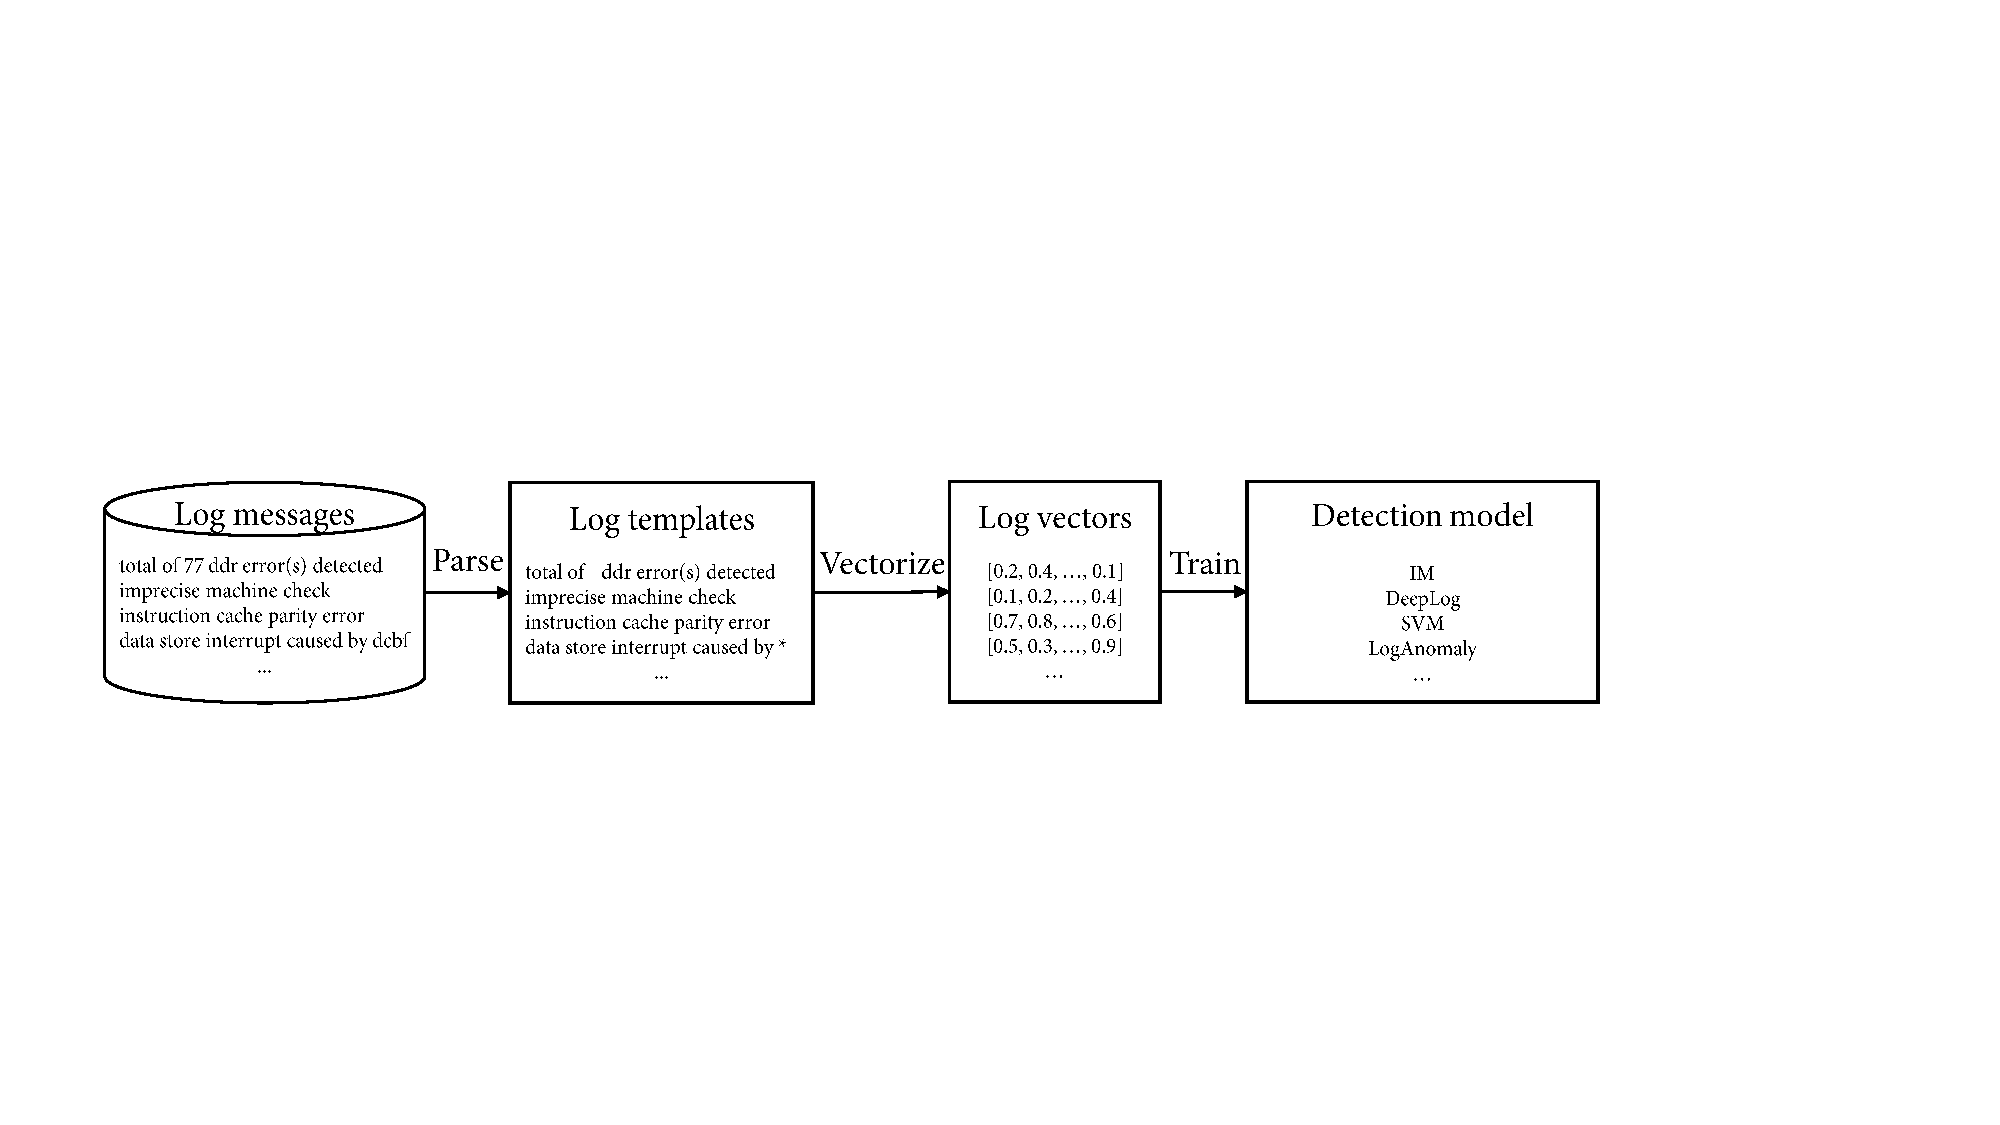
\includegraphics[width=1.0\textwidth]{gfx/chap5/traditionaloverviewlogs.pdf}}
\caption{Overview of traditional log anomaly detection approaches.}
\label{fig:parsingreferenceanomaly}
\end{figure}

In this chapter, we analyze the detection of system anomalies from log data. A plethora of methods exist to address some of the challenges posed by log data and complex systems  (~\cite{du2017deeplog,zhang2019robust,meng2019loganomaly,shilinpca}). A common characteristic is that they follow similar pipelines, depicted in Figure~\ref{fig:parsingreferenceanomaly}. (1) Owing to the unstructured nature of logs, the first crucial step is to parse log messages into structured more abstract data (e.g., templates, activities) for a subsequent analysis. (2) Vectorization of the parsed logs (i.e., the templates) is performed where they are converted into a vector form (e.g., one-hot encoding~\cite{Goodfellow-et-al-2016} or term frequency encoding~\cite{ramos2003using}). (3) The logs are utilized for training of the detection models (e.g., DeepLog~\cite{du2017deeplog}). 

The traditional log anomaly detection pipelines suggest that the log parsing, log vectorization, and detection model directly impact the effectiveness~\cite{zhu2019tools,meng2019loganomaly}.

\begin{enumerate}
    \item Even small errors, such as 4\%, in parsing could cause a performance reduction of one order of magnitude in log anomaly detection (from 40\% to 3.7\%)~\cite{he2016evaluation}.
    \item The vector representation of the log messages (log vectors) particularly affects the generalization of the models on unseen log messages, which is of importance in systems with frequent updates~\cite{zhang2019robust,meng2019loganomaly}.
    \item The models need to be sufficiently powerful and expressive to extract patterns from the potentially high-dimensional log vectors. 
\end{enumerate}

This chapter presents methods that cover these aspects in support to an effective anomaly detection.

% Therefore, first we present a novel parsing method, denoted as NuLog, which directly affects the performances of numerous methods that base their anomaly detection on the parsed log templates~\cite{du2017deeplog,meng2019loganomaly,zhang2019robust,shilinpca}. In the second part of this chapter, we present a novel log anomaly detection method, denoted as Logsy. It aims to improve the log representation, and thus the anomaly detection. In Logsy, the challenge of learning meaningful log representations is addressed directly with the optimization of novel spherical loss function. Aiming to obtain a better log representations, implicitly, we shift from the traditional anomaly detection pipeline. Logsy is able to learn the log parsing and vectorization jointly with an anomaly score in an end-to-end fashion.

We summarize the contributions in this chapter below \footnote{Parts of this chapter are published in~\cite{nedelkoski2020loganomaly,nedelkoski2020selfsupervised,nedelkoski2020data,nedelkoski2020bigdatatransfer}.}.
\begin{itemize}
    \item Novel neural log parser for log anomaly detection, denoted as NuLog~\cite{nedelkoski2020selfsupervised}, which not only parses the log messages, but also provides log vector representations.
    \item We illustrate two use cases using NuLog variants, for supervised and unsupervised anomaly detection. However, we observe a large gap between the supervised and unsupervised anomaly detection methods owing to the imperfect log representations.
    \item To bridge the gap between the supervised and unsupervised methods, we present Logsy~\cite{nedelkoski2020loganomaly}, a novel method with a spherical classification loss function for log anomaly detection.
    \item We demonstrate the key features of Logsy including utilizing log vector representations in related methods and adding expert knowledge, if available.
\end{itemize}

\section{Log parsing}\label{ch:logs:logparsing}
The content of a log record is semi-structured text, which contain tags (e.g., timestamp and service name) and free-text written by software developers. Often, the tagged data are relatively simple to parse, while the free-form text is challenging~\cite{he2017drain,zhu2019tools}. The free text is a composition of constant string templates and variable values. The template is the logging instruction (e.g., \textit{print()}, \textit{log.info()}) from which the log message is produced. The objective of a log parser is the transformation of the unstructured free text into a structured log template and associated list of variables. For example, the template \textit{"Attempting claim: memory $\langle * \rangle$ MB, disk $\langle * \rangle$ GB, vcpus $\langle * \rangle$ CPU"} is associated with the variable list \textit{["2048", "20, "1"]}, where $\langle * \rangle$ denotes the position of each variable and is connected with the positions of the values within the list. The variable list can be empty if the template does not contain variable parts. We illustrate the log parsing task in Figure~\ref{fig:log_parsing_task}.

\begin{figure}[htbp]
\centerline{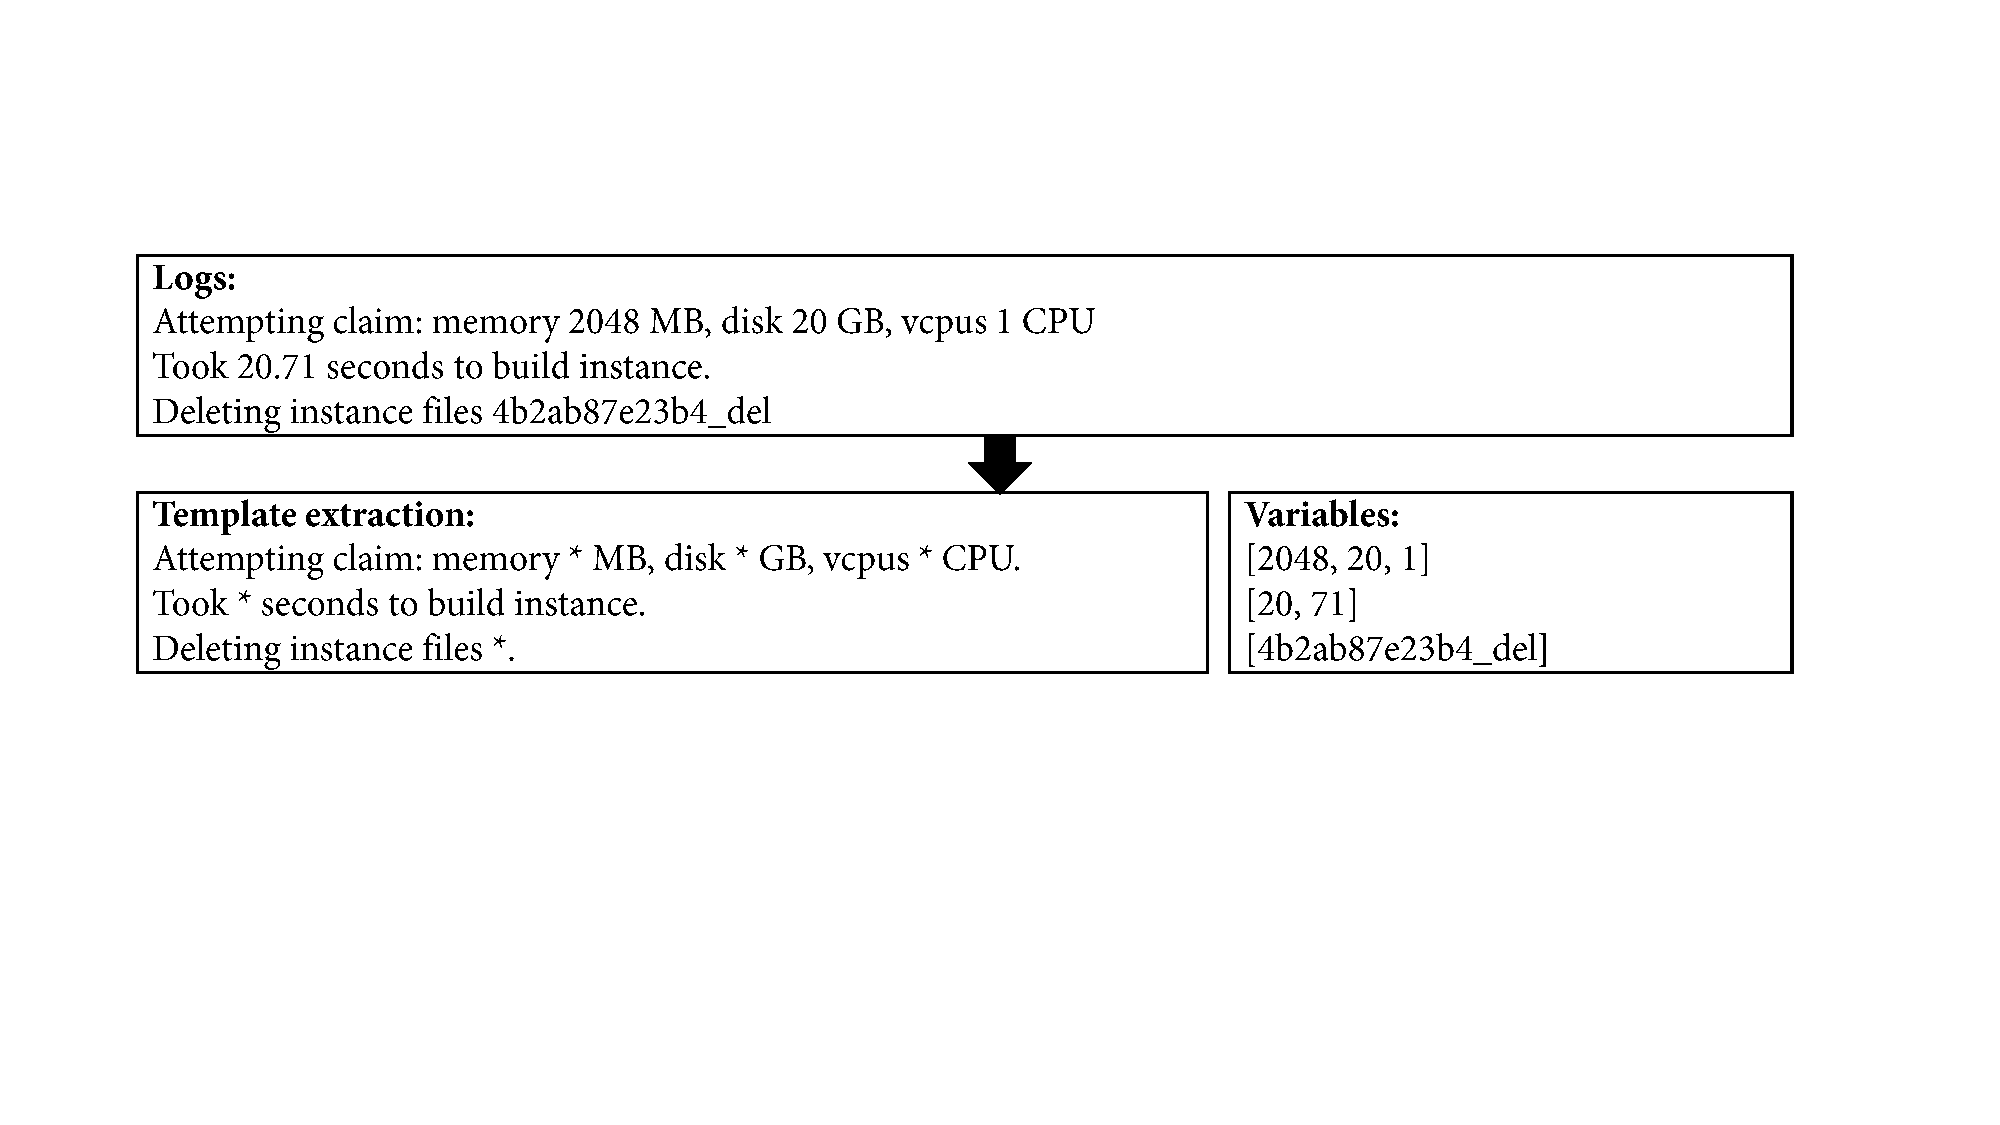
\includegraphics[width=1.0\textwidth]{gfx/chap5/log_parsing_task.pdf}}
\caption{Examples of system logs and their templates.}
\label{fig:log_parsing_task}
\end{figure}

Traditional log parsing techniques rely on regular expressions designed and maintained by human experts. This manual task is difficult to achieve in large systems consisting of diverse software and hardware components. Additionally, frequent software updates necessitate constant checking and adjustment of these statements, which is a tedious error-prone task. Related log parsing methods~\cite{he2017drain, du2016spell,hamooni2016logmine,zhu2017deep,imweber2015} depend on manual human interventions, parse trees, heuristics, and domain knowledge. Analyses of the performances of existing log parsing methods on various systems reveal their lack of robustness to produce consistently good parsing results~\cite{zhu2019tools}. 
This implies the necessity to choose a parsing method for the application or system at hand and incorporate domain-specific knowledge. In such case, operators of large distributed software systems are faced with overhead of managing different parsing methods for their components whereof each need to be accordingly understood and tuned. 

Notably, log parsing methods have to be accurate on log data from various systems, from applications on mobile operating systems to cloud infrastructure management platforms, with minimal human intervention.

After parsing, the parsed templates are transformed to log vectors for anomaly detection. The described procedures to generate log template vectors may introduce additional uncertainty and complexity. Therefore, it is desirable to incorporate the task of generating log vectors into the parsing procedure. Such a log parsing approach would meet the requirements of recent log analysis methods~\cite{meng2019loganomaly,huang2020hitanomaly,zhang2019robust}, avoid the additional external log vector generators, and provide new possibilities for log analysis tasks.

To this end, we present NuLog. We formulate the learning task on the observation that the presence of a word on a particular position in a log message is conditioned on its context. Inspired by the Cloze procedure~\cite{taylor1953cloze}, the task is carried out by masking the word that the model needs to learn to predict. In this manner, the model is forced to learn the appearance of the word within its context. The key idea for parsing is that the correct prediction of the masked word implies that the word is a part of the log template. Otherwise, it is a parameter (variable). The advantages of this approach are that it can produce both log template and numerical vector sumarization and enable downstream tasks such as anomaly detection. With the introduction of NuLog, we modify the traditional log anomaly detection pipeline illustrated in Figure~\ref{fig:parsingreferenceanomaly} to include the log parsing and vectorization within the same block. We describe NuLog in detail below.

\section{\textit{NuLog}: neural log parsing}\label{methodology}
In this section, we define the terminology, present the model, and demonstrate an approach to extract log templates and numerical log vector representations. In addition, an evaluation of the parsing method is presented.

We define a log as a sequence of temporally ordered unstructured text messages $L=(\mathbf{l_{i}} \,:\,i=1,2,...)$, where each message $\mathbf{l_{i}}$ is generated by a logging instruction within the software source code and $i$ is its positional index within the sequence. 

The smallest inseparable singleton object within a log message is token. Each log message consists of a finite sequence of tokens, $\mathbf{r_i}=(w_{j}\,:\,w \in  \mathbb{V},\,j=1,2,..., ms_i)$, where $ \mathbb{V}$ is a set (vocabulary) of all tokens, $j$ is the positional index of a token within the log message, and $ms_i$ is the total number of tokens in $\mathbf{l_i}$. We use $\vert r_i \vert$ instead of $ms_i$ in the following analysis. For different $\mathbf{l_i}$, $\vert \mathbf{r_i} \vert$ can vary. Depending on the concrete tokenization method, $w_j$ can be a word, word piece, or character. Therefore, the tokenization is defined as a transformation function $\mathcal{T}: \mathbf{l_i} \to \mathbf{r_i}, \forall i$.

The notions of context and numerical vector representation (embedding vector) are additionally introduced. For a token $w_j$, its context is defined by preceding and subsequent sequences of tokens, i.e., tuple of sequences: $C(w_j)=((w_{1}, w_{2},...,w_{j-1}), \allowbreak (w_{j+1}, w_{j+2},...,w_{\vert \mathbf{r_i} \vert}))$, where $0 \leq j \leq \vert \mathbf{r_i} \vert$. Each token is represented through an embedding vector in a $d$-dimensional space $\mathbf{x_j} \in \mathbb{R}^{d}$ of either token or log message. Therefore, we define the log message $\mathbf{x_i}=\{x_0,x_1,\dots,x_{|r_i|}\}$, where each token is represented as a vector.

\subsection{Parsing with Transformers}\label{NuLog}

NuLog is composed of preprocessing (tokenization and masking), modeling, and template extraction. The overall architecture based on an example log message input is depicted in Figure~\ref{fig:nulog}. The raw log messages are tokenized, where an \texttt{EMBEDDING} token is inserted at the first position. Using a dictionary, each token is then replaced with an index. As the last step, the masking of the tokens is performed, where the masked token is used as a target for prediction. As each token in the model is represented in vector form (indices are mapped to vectors), the \texttt{EMBEDDING} token is later used to summarize the log message from the respective token embeddings. The tokens are fed into the model, where parameters are optimized by minimizing the cross entropy loss between the target and predicted masked token. Finally, the trained model is used to extract log templates and numerical vector representation $\mathbf{z}$.

\begin{figure}[!t]
\centerline{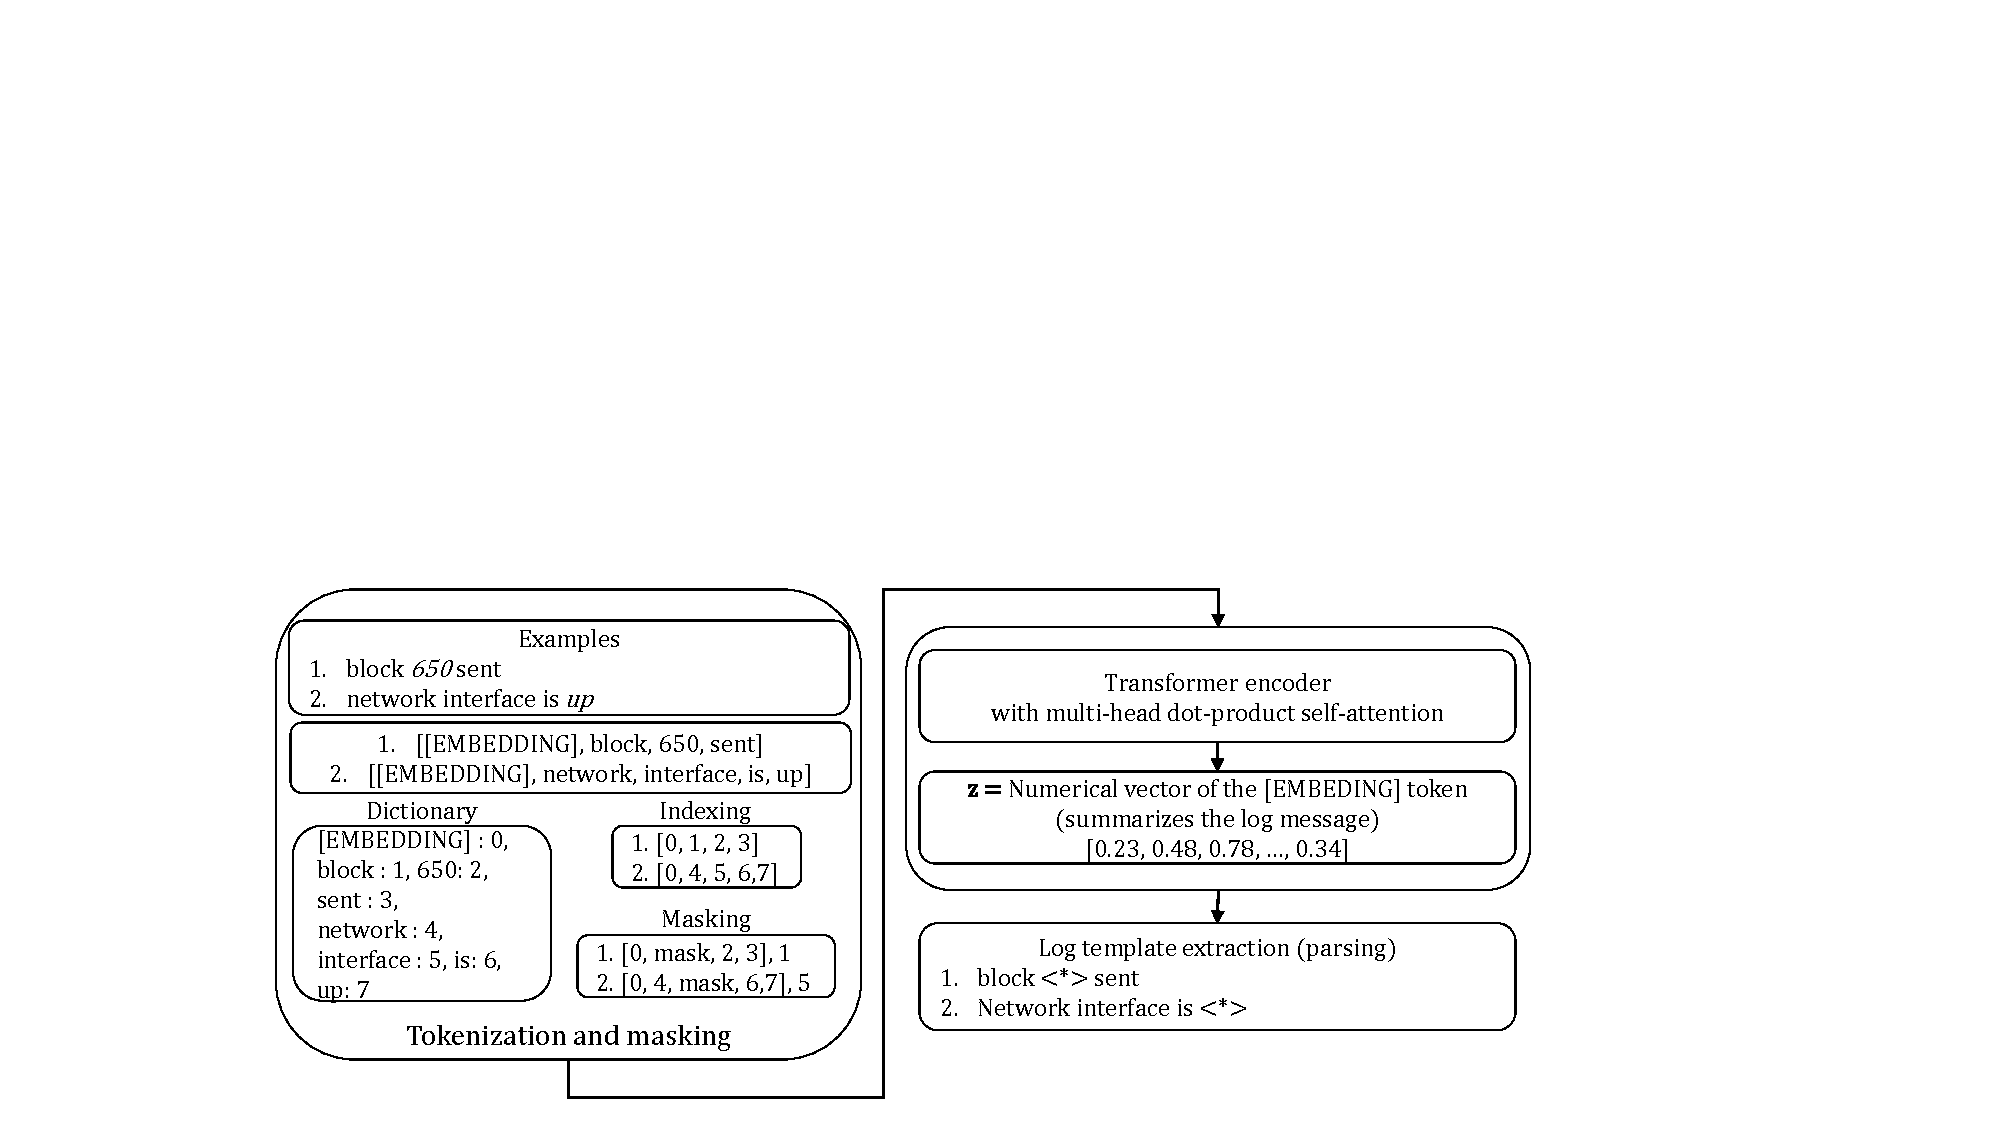
\includegraphics[width=1.0\textwidth]{gfx/chap5/nulog.pdf}}
\caption{Overview of the NuLog architecture.}
\label{fig:nulog}
\end{figure}

\textbf{Tokenization.} Tokenization transforms each log message into a sequence of tokens. For NuLog, we utilize a simple filter-based splitting criterion (e.g., on a white space) to perform a string split operation. In Figure~\ref{fig:nulog}, we illustrate the tokenization of two log messages. In contrast to related approaches~\cite{zhu2019tools} that utilize additional hand-crafted regular expressions to parse IP addresses, numbers, and URLs, NuLog does not change the original log messages at this stage. Such approaches are error-prone and require manual adjustments in different systems and updates within the same system. NuLog utilizes the appearance of the tokens within a context. These parameters (e.g., IP addresses) are assigned with a low probability as they are not constant within a particular context.

\textbf{Masking.} The concept behind the proposed parsing method is to learn a general semantic representation of the log data by analyzing occurrences of tokens within their context. We apply an approach referred to as masked language modeling (MLM). Our masking module uses the output of the tokenization step as an input, which is a token sequence of a log message. A percentage of tokens from the sequence are randomly chosen and replaced by the special \texttt{$\langle MASK \rangle$} token. If the percentage suggests replacing two tokens with masks, the masking module will create two samples, where each of the words will be masked once. In Figure~\ref{fig:nulog}, the masking is performed only on one token. Therefore, one masked log message is created. The masked token sequence is used as an input for the model, while the masked token acts as the prediction target. Furthermore, we apply padding with \texttt{PAD} tokens. The padding is applied to the maximal number of tokens across all log messages in the dataset to create evenly sized inputs.

\textbf{Model}. The method has two operation modes, offline and online. During the offline phase, log messages are used to tune all model parameters through back-propagation. During the online phase, every log message is passed forward through the model. This generates the corresponding log template and embedding vector for each log message.


\begin{figure}[!t]
\centerline{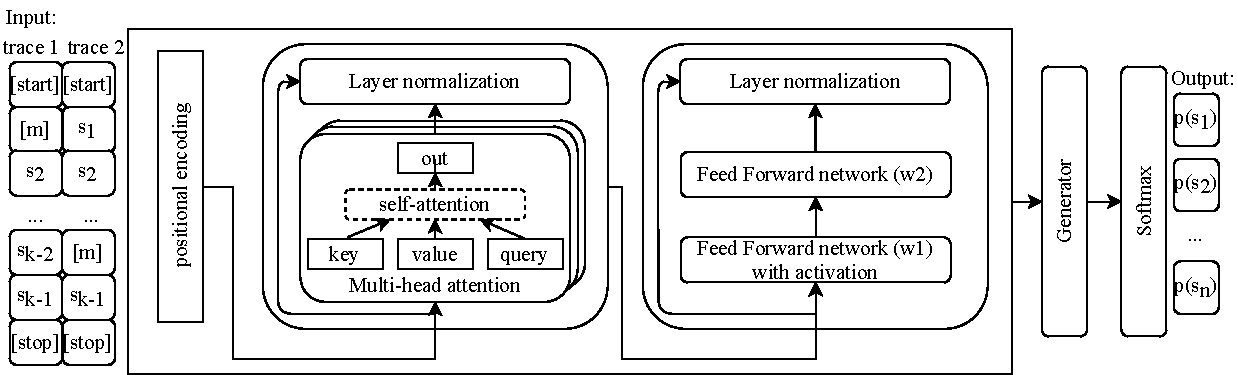
\includegraphics[width=\textwidth]{gfx/chap5/nulogtransformer.pdf}}
\caption{Model architecture of \texttt{NuLog} for parsing of the logs.}
\label{fig:2}
\end{figure}

Figure~\ref{fig:2} depicts the complete architecture. We base the model's architecture on the Transformer model~\cite{vaswani2017attention}. The Transformer network obtains word/token vectors as a weighted sum of the vectors produced by the others tokens. It attends to tokens that are similar and combines them to obtain a new representation. The model applies two operations on the input token vectors, token vectorization and positional encoding. The subsequent encoder structure uses the result of these operations as an input. It is composed of two elements, a self-attention layer and feedforward layer. The last model component is a single linear layer with a softmax activation over all tokens appearing in the logs. We provide a detailed explanation of each model element below.

As all subsequent elements of the model expect numerical inputs, we initially transform the tokens into randomly initialized numerical vectors $\mathbf{x} \in \mathbb{R}^d$. These vectors are referred to as token embeddings and are a part of the training process, which implies that they are adjusted during the training to represent the semantic meaning of tokens depending on their context. These numerical token embeddings are passed to the positional encoding block. In contrast to, e.g., recurrent architectures, attention-based models do not contain any notion of input order. Therefore, this information needs to be explicitly encoded and merged with the input vectors to consider their position within the log message. This block calculates a vector $\mathbf{p} \in \mathbb{R}^d$ representing the relative position of a token based on sine and cosine functions,
%We follow the recommendations of~\cite{vaswani2017attention} and employ the following equations for positional embeddings calculation

\begin{equation}\label{eq:sincosin}
    p_{2k}=sin \left( \frac{j}{10000^{\frac{2k}{v}}} \right), \;\;
    p_{2k+1}=cos \left( \frac{j}{10000^{\frac{2k + 1}{v}}} \right),
\end{equation}

where $k=0,1,\dots,d-1$ is the index of each element in $\mathbf{p}$ and $j=1,2,\dots,M$ is the positional index of each token. The parameter $k$ describes the exponential relationship between each value of vector $\mathbf{p}$. Additionally, sine and cosine functions are interchangeably applied. Both enable a better discrimination of the respective values within a specific vector of $\mathbf{p}$. Furthermore, both functions approximately linearly depended on the position parameter $j$, which was hypothesized so that the model can easily attend at the respective positions. Finally, both vectors can be combined as $\mathbf{x'} = \mathbf{x} + \mathbf{p}$. The values for the frequency of the sine and cosine functions were obtained empirically, as in ~\cite{vaswani2017attention}.

The encoder block of our model starts with a multi-head attention element, where a softmax distribution over the token embeddings is calculated. Intuitively, it describes the significance of each embedding vector for the prediction of the target masked token. We summarize all token embedding vectors as rows of a matrix $X'$ and apply the following formula,
\begin{equation}
    X''_l=softmax \left( \frac{Q_l \times K^T_l}{\sqrt{w}} \right) \times V_l, \; \text{for} \; l = 1, 2, \dots, L,
\end{equation}
where $L$ denotes the number of attention heads, $w = \frac{d}{L}$, and $d \, \text{mod} \, L = 0$. The parameters $Q$, $K$, and $V$ are matrices, which correspond to the query, key, and value elements in Figure~\ref{fig:2}, respectively. They are obtained by applying matrix multiplications between the input $X'$ and respective learnable weight matrices $W_{l}^{Q}$, $W_{l}^{K}$, $W_{l}^{V}$,

\begin{equation}
    Q_l= X' \times W_{l}^{Q}, \; K_l= X' \times W_{l}^{K}, \; V_l= X' \times W_{l}^{V},
\end{equation}

where $W_{l}^{Q}, \; W_{l}^{K}, \; W_{l}^{V} \in \mathbb{R}^{M \times w}$. The division by $\sqrt{w}$ stabilizes the gradients during the training~\cite{vaswani2017attention}. The softmax function is then applied and the result is used to scale each token embedding vector $V_{l}$. The scaled matrices $X''_l$ are concatenated to a single matrix $X''$ with a size of $M \times d$. As depicted in Figure~\ref{fig:2}, a residual connection between the input token matrix $X'$ and its respective attention transformation $X''$ exists, followed by a normalization layer $norm$. These are used to improve the performance of the model by addressing different potential problems during the learning such as small gradients and covariate shift phenomena. In this manner, the original input is updated by the attention-transformed equivalent, $X' = norm(X' + X'')$.

The last element of the encoder consists of two feed-forward linear layers with a ReLU activation between them. It is applied individually on each row of $X'$. Thereby, identical weights for every row are used, which can be described as a convolution over each attention-transformed matrix row with a kernel size of one. This step serves as an additional information enrichment for the embeddings. A residual connection followed by a normalization layer between the input matrix and output of both layers is employed. This model element preserves the dimensionality $X'$.

The final element of the model consists of a single linear layer. It receives the encoder result $X'$ and extracts the token embedding vector of the \texttt{EMBEDDING} token. As every log message token sequence is prepadded by this special token, it is the first row of the matrix, i.e., $\mathbf{x'_0} \in X'$. The linear layer maps this vector with a size of $d$ to a vector whose size corresponds to the total number of tokens $|\mathbb{T}|$ in the dataset. The subsequent softmax is utilized to calculate the probability distribution over each element of $\mathbb{T}$. During the training with a cross-entropy loss function, the masked token is used as the target to be predicted. As the last vector embedding of the \texttt{EMBEDDING} token is used for prediction, it summarizes the log message. We hypothesize that the constant part of log templates will constraint the model to learn similar \texttt{EMBEDDING} vectors when log messages are from the same template. This leads to mapping of the log messages to their vector representation, which can enable other downstream log analysis tasks.

\newpage

\subsection{Log template and vector extraction}
After the model is trained, the extraction of all log templates within a log dataset is executed online. Each log message is used as an input and the masking module is configured such that every token is masked consecutively, one at a time. We measure the model's ability to predict each token, and thus decide whether the token is a constant part of the template or variable. A high confidence in the prediction of a specific token indicates a constant part of the template. A low confidence is interpreted as a variable. We employed the following procedure. If the prediction of a particular token is in the top $\epsilon$ predictions and does not contain numbers, we consider it a constant part of the template; otherwise, we considered it a variable. For each variable, an indicator \texttt{$\langle * \rangle$} is placed on its position within the log message.

Once the templates are obtained, to perform anomaly detection, we follow the traditional log anomaly detection pipeline described above.

% The computational complexity for parsing one log message $\mathbf{t_i}$ is $\mathcal{O}(\text{max}_{i}|\mathbf{t_i}|)$ + $\mathcal{O}(\text{max}_{i}|\mathbf{t_i}|)$ + $\mathcal{O}(1)$ + $\mathcal{O}(|\mathbb{T}|\log \mathbb{T})$, for tokenization, masking, forward pass, and top-k sorting, where $\text{max}_{i}|\mathbf{t_i}|$ is the maximum number of tokens in the log messages and $|\mathbb{T}|$ is the size of the set of all tokens. This makes our method in worst case $\mathcal{O}(|\mathbb{T}|\log \mathbb{T})$

Another contribution of NuLog is that we enable generation of a vector representation of the log messages. The~\texttt{EMBEDDING} token attends over all tokens in the log. Hence, it embeds information of all of them without being biased toward any of the original log tokens. Moreover, it encodes semantic information inside the logs. This leads to one-to-one mapping between the log message type and vector representation of the \texttt{EMBEDDING} token. 

\subsection{NuLog: Evaluation}\label{nulog:evaluation}
To quantify the effectiveness of \texttt{NuLog} in the task of log parsing, we evaluate it on 10 presented datasets and compare it to 12 existing log parsing methods. We reproduce the results of the parsing benchmark~\cite{zhu2019tools} for all log parsers and include NuLog's results. All parsers and their parameters are tuned to achieve their best performances.

% \begin{table}[!t]
% \centering
% \caption{Datasets and \texttt{NuLog} hyperparameter setting.}
% % \resizebox{\columnwidth}{!}{%
% \begin{tabular}{llcc}
% \hline
% System   & T   & epochs & $\epsilon$   \\ \hline
% BGL      &120 & 3        & 50  \\
% Android  &166  & 5        & 25  \\
% OpenStack&43  & 6        & 5   \\
% HDFS     &14  & 5        & 15  \\
% Apache   &6  & 5        & 12  \\
% HPC      &46 & 3        & 10  \\
% Windows  &50  & 5        & 95  \\
% HealthApp&75  & 5        & 100 \\
% Mac      &341 & 10       & 300 \\
% Spark    &36  & 3        & 50  \\ \hline
% \end{tabular}
% % }
% \label{table:hyperparameters}
% \end{table}

\subsubsection{Datasets}\label{Datasets}
The log datasets employed in our experiments consist of: (1) supercomputer logs, Blue Gene L (BGL) and HPC, (2) distributed system logs, Hadoop distributed file system (HDFS), OpenStack, and Spark, and (3) standalone software logs, Apache, Windows, Mac, and Android. To enable reproducibility, we follow the guidelines of Zhu et al.~\cite{zhu2019tools} and utilize a random sample of 2000 log messages from each dataset, where the ground truth templates are available. 

\subsubsection{Evaluation metrics}
For comparability of NuLog to the previous methods~\cite{zhu2019tools}, we utilize the benchmark PA metric. It is defined as the ratio of correctly parsed log messages to the total number of log messages. A log message is considered correctly parsed if its log template corresponds to the same group of log messages as that of the ground truth. For example, if a log sequence $[e_1, e_2, e_2]$ is parsed to $[e_1, e_4, e_5]$, we obtain $PA=\frac{1}{3}$ as the second and third messages are not grouped together. The parsing accuracy does not measure the string matching between the template and ground truth. Therefore, we enrich the evaluation with an additional metric, the edit distance. This can be used to quantify the dissimilarity between two log templates by counting the minimum number of operations required to transform one into the other.




\begin{table}[htbp]
\centering
\caption{Comparisons of log parsers and our method \texttt{NuLog} in terms of PA.}
\resizebox{\columnwidth}{!}{%
\begin{tabular}{|l|cccccccccccccc|}
\hline
Dataset   & SLCT           & AEL            & LKE   & LFA            & LogSig & SHISHO & LogCluster & LenMa & LogMine        & Spell          & Drain          & MoLFI & BoA          & NuLog           \\ \hline 
HDFS      & 0.545          & 0.998          & 1.000 & 0.885          & 0.850  & 0.998  & 0.546      & 0.998 & 0.851          & 1.000          & 0.998          & 0.998 & \textbf{1.000} & 0.998          \\
Spark     & 0.685          & 0.905          & 0.634 & \textbf{0.994} & 0.544  & 0.906  & 0.799      & 0.884 & 0.576          & 0.905          & 0.920          & 0.418 & 0.994          & \textbf{1.000} \\
OpenStack & \textbf{0.867} & 0.758          & 0.787 & 0.200          & 0.200  & 0.722  & 0.696      & 0.743 & 0.743          & 0.764          & 0.733          & 0.213 & 0.867          & \textbf{0.990} \\
BGL       & 0.573          & 0.758          & 0.128 & 0.854          & 0.227  & 0.711  & 0.835      & 0.690 & 0.723          & 0.787          & \textbf{0.963} & 0.960 & 0.963          & \textbf{0.980} \\
HPC       & 0.839          & \textbf{0.903} & 0.574 & 0.817          & 0.354  & 0.325  & 0.788      & 0.830 & 0.784          & 0.654          & 0.887          & 0.824 & 0.903          & \textbf{0.945} \\
Windows   & 0.697          & 0.690          & 0.990 & 0.588          & 0.689  & 0.701  & 0.713      & 0.566 & 0.993          & 0.989          & \textbf{0.997} & 0.406 & 0.997          & \textbf{0.998} \\
Mac       & 0.558          & 0.764          & 0.369 & 0.599          & 0.478  & 0.595  & 0.604      & 0.698 & \textbf{0.872} & 0.757          & 0.787          & 0.636 & \textbf{0.872} & 0.821          \\
Android   & 0.882          & 0.682          & 0.909 & 0.616          & 0.548  & 0.585  & 0.798      & 0.880 & 0.504          & \textbf{0.919} & 0.911          & 0.788 & \textbf{0.919} & 0.827          \\
HealthApp & 0.331          & 0.568          & 0.592 & 0.549          & 0.235  & 0.397  & 0.531      & 0.174 & 0.684          & 0.639          & \textbf{0.780} & 0.440 & 0.780          & \textbf{0.875} \\
Apache    & 0.731          & 1.000          & 1.000 & 1.000          & 1.000  & 1.000  & 0.709      & 1.000 & 1.000          & 1.000          & 1.000          & 1.000 & \textbf{1.000} & \textbf{1.000} \\ \hline
\end{tabular}
}
\label{table:comparisonPA}
\end{table}



\subsubsection{Parsing results}

\textbf{Parsing accuracy} results are presented in Table~\ref{table:comparisonPA}. Each row contains the datasets while the compared methods are presented in the table columns. The penultimate column contains the highest value of the first twelve columns, referred to as best of all, while the last column contains the results for \texttt{NuLog}. The values in bold indicate the best of the methods per dataset. HDFS and Apache datasets are most frequently parsed with a PA of 100\%, because HDFS and Apache error logs have relatively unambiguous event templates, which are simple to identify. For them, \texttt{NuLog} achieves comparable results. For the Spark, BGL, and Windows datasets, the existing methods already achieve high PA values above 96\% (BGL) or above 99\% (Spark and Windows). Our method can slightly outperform these methods. For the rather complex log data from OpenStack, HPC, and HealthApp, the baseline methods achieve a PA between 78\% and 90\%, which are significantly outperformed by \texttt{NuLog} by 4--13\%.

With the proposed method, we explicitly aim to support a broad range of diverse log data types. Therefore, the robustness of \texttt{NuLog} is analyzed and compared to those of the related methods. Figure~\ref{robustness_pa} shows the accuracy distribution of each log parser across the log datasets within a boxplot. From left to right in the figure, the log parsers are arranged in ascending order of the median PA. LogSig has the lowest, while \texttt{NuLog} has the highest median PA. Although most log parsing methods achieve high PA values of 90\% for specific log datasets, they have large variances when applied across all given log types. \texttt{NuLog} outperforms the other baseline methods in terms of PA robustness with a median of 0.99, which is even above the best of all medians of 0.94.

\begin{figure}[!t]
\centerline{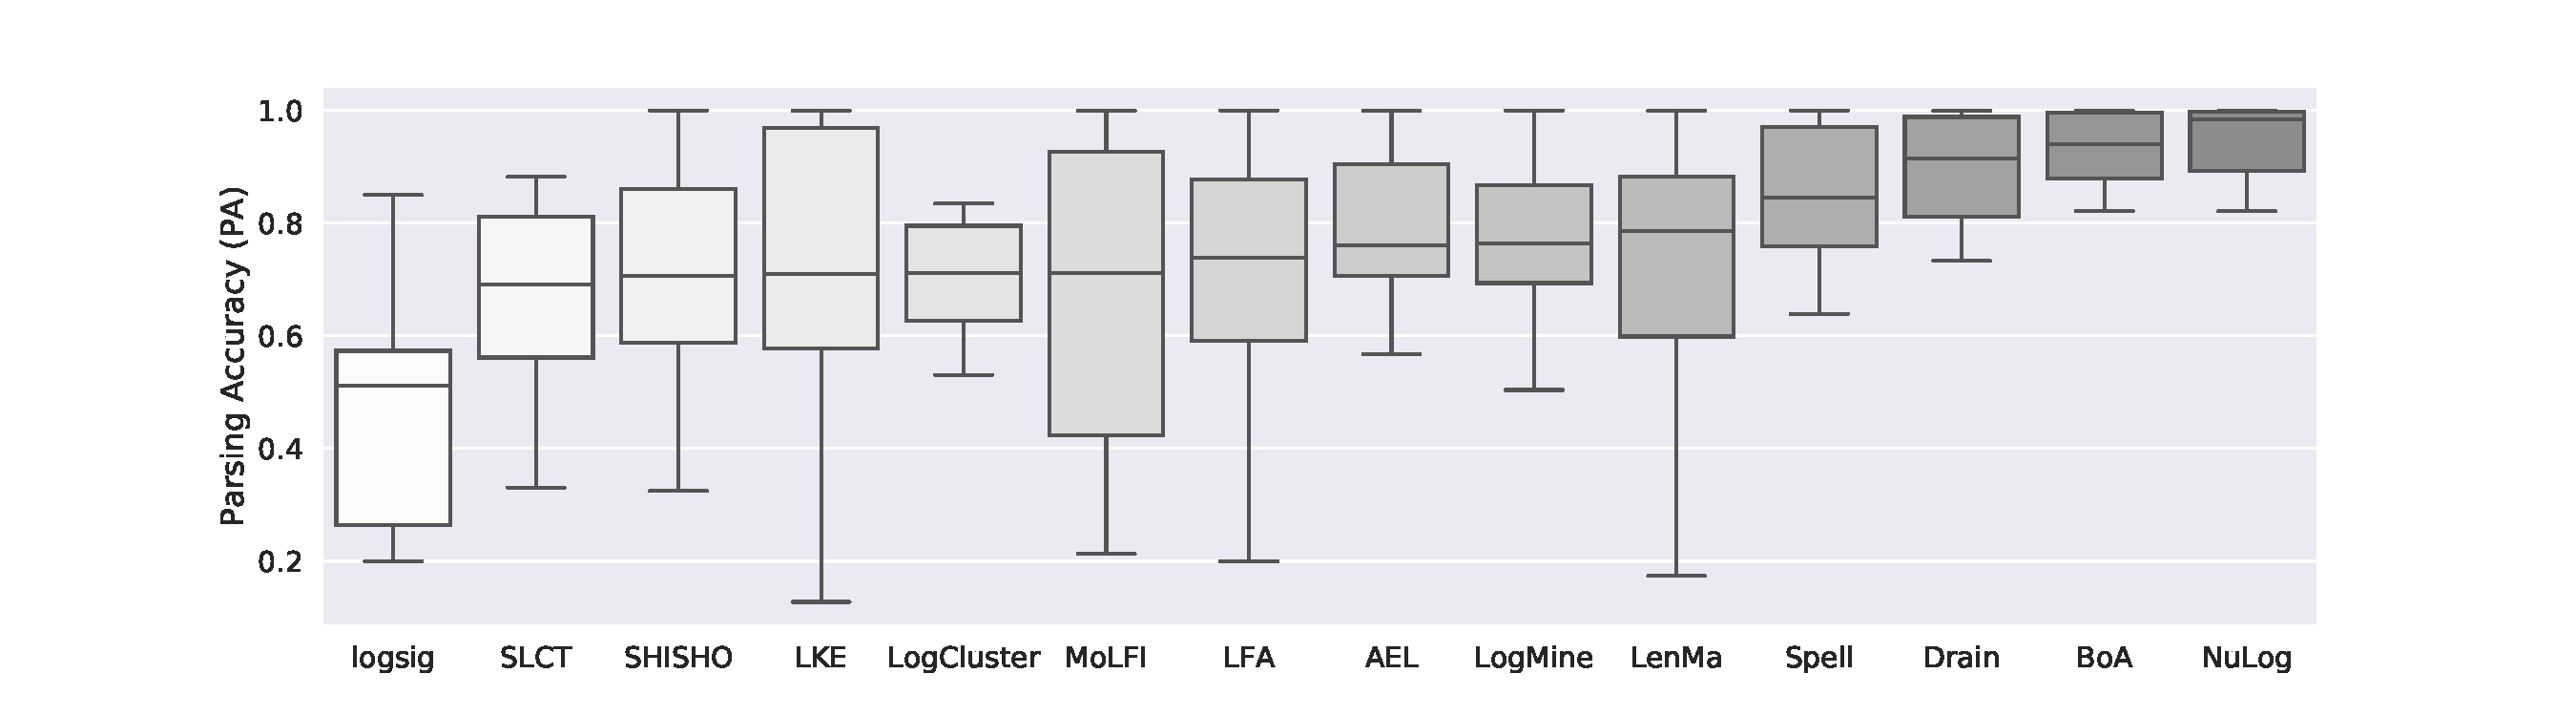
\includegraphics[width=1.0\textwidth]{gfx/chap4/robustness.pdf}}
\caption{Robustness evaluation of the PA of the log parsers.}
\label{robustness_pa}
\end{figure}

\begin{table}[!htbp]
\centering
\caption{Comparisons of log parsers and our method \texttt{NuLog} in terms of edit distance.}
\resizebox{\columnwidth}{!}{%
\begin{tabular}{|l|cccccccccccccc|}
\hline
Dataset &  LogSig &      LKE &    MoLFI &     SLCT &      LFA &  LogCluster &   SHISHO &  LogMine &    LenMa &    Spell &      AEL &    Drain  &  BoA&    NuLog \\
\hline 
HDFS & 19.1595 &  17.9405 &  19.8430 &  13.6410 &  30.8190 &     28.3405 &  10.1145 &  16.2495 &  10.7620 &   9.2740 &   8.8200 &   8.8195 &    8.8195& \textbf{3.2040} \\
Spark & 13.0615 &  41.9175 &  14.1880 &   6.0275 &   9.1785 &     17.0820 &   7.9100 &  16.0040 &  10.9450 &   6.1290 &   3.8610 &   \textbf{3.5325} &  3.5325&  12.0800 \\
BGL &  11.5420 &  12.5820 &  10.9250 &   9.8410 &  12.5240 &     12.9550 &   8.6305 &  19.2710 &   8.3730 &   7.9005 &   5.0140 &   \textbf{4.9295} &   4.9295&  5.5230 \\
HPC &  4.4475 &   7.6490 &   3.8710 &   2.6250 &   3.1825 &      3.5795 &   7.8535 &   3.2185 &   2.9055 &   5.1290 &   \textbf{1.4050} &   2.0155 &   1.4050&      2.9595 \\
Windows &  7.6645 &  11.8335 &  14.1630 &   7.0065 &  10.2385 &      6.9670 &   5.6245 &   6.9190 &  20.6615 &   4.4055 &  11.9750 &   6.1720 &   5.6245&     \textbf{4.4860} \\
Android & 16.9295 &  12.3505 &  39.2700 &   3.7580 &   9.9980 &     16.4175 &  10.1505 &  22.5325 &   3.2555 &   8.6680 &   6.6550 &   3.2210 &    3.2210&    \textbf{1.1905} \\
HealthApp & 17.1120 &  14.6675 &  21.6485 &  16.2365 &  20.2740 &     16.8455 &  24.4310 &  19.5045 &  16.5390 &   8.5345 &  19.0870 &  18.4965 &    14.6675&  \textbf{6.2075} \\
Apache & 14.4420 &  14.7115 &  18.4410 &  11.0260 &  10.3675 &     16.2765 &  12.4405 &  10.2655 &  13.5520 &  10.2335 &  10.2175 &  \textbf{10.2175} &   10.2175& 11.6915 \\
OpenStack & 21.8810 &  29.1730 &  67.8850 &  20.9855 &  28.1385 &     31.4860 &  18.5820 &  23.9795 &  18.5350 &  27.9840 &  \textbf{17.1425} &  28.3855 &   17.1425&  21.2605 \\
Mac & 27.9230 &  79.6790 &  28.7160 &  34.5600 &  41.8040 &     21.3275 &  19.8105 &  17.0620 &  19.9835 &  22.5930 &  19.5340 &  19.8815 &      17.062& \textbf{2.8920} \\
\hline
\end{tabular}
}

\label{table:edit_distance}
\end{table}


\textbf{Edit distance} scores are listed in Table~\ref{table:edit_distance}. The table structure is the same as that of the PA results. The value in bold indicates the best edit distance across all tested methods per dataset. In terms of edit distance, \texttt{NuLog} outperforms the existing methods on the HDFS, Windows, Android, HealthApp, and Mac datasets. Its performance is comparable on the BGL, HPC, Apache, and OpenStack datasets. It achieves a larger edit distance on the Spark log data.

We verify the robustness in terms of edit distance across the different log datasets. Figure~\ref{robustness_ed} shows a box-plot of the edit distance distribution of each log parser for all log datasets. From left to right in the figure, the log parsing methods are arranged in descending order of the median edit distance. Again, although most log parsing methods achieve minimal edit distance scores under 10, most of them have large variances over different datasets and are thus not generally applicable for diverse log data types. MoLFI has the largest median edit distance, while Spell and Drain exhibit small median edit distances for multiple datasets. NuLog outperforms the state-of-the-art models, with the smallest edit distance values with a median of 5.00, which is smaller than the best-of-all median of 7.22.

These results show that NuLog parses the log messages accurately, while preserving the string structure of the message.


\begin{figure}[!htbp]
\centerline{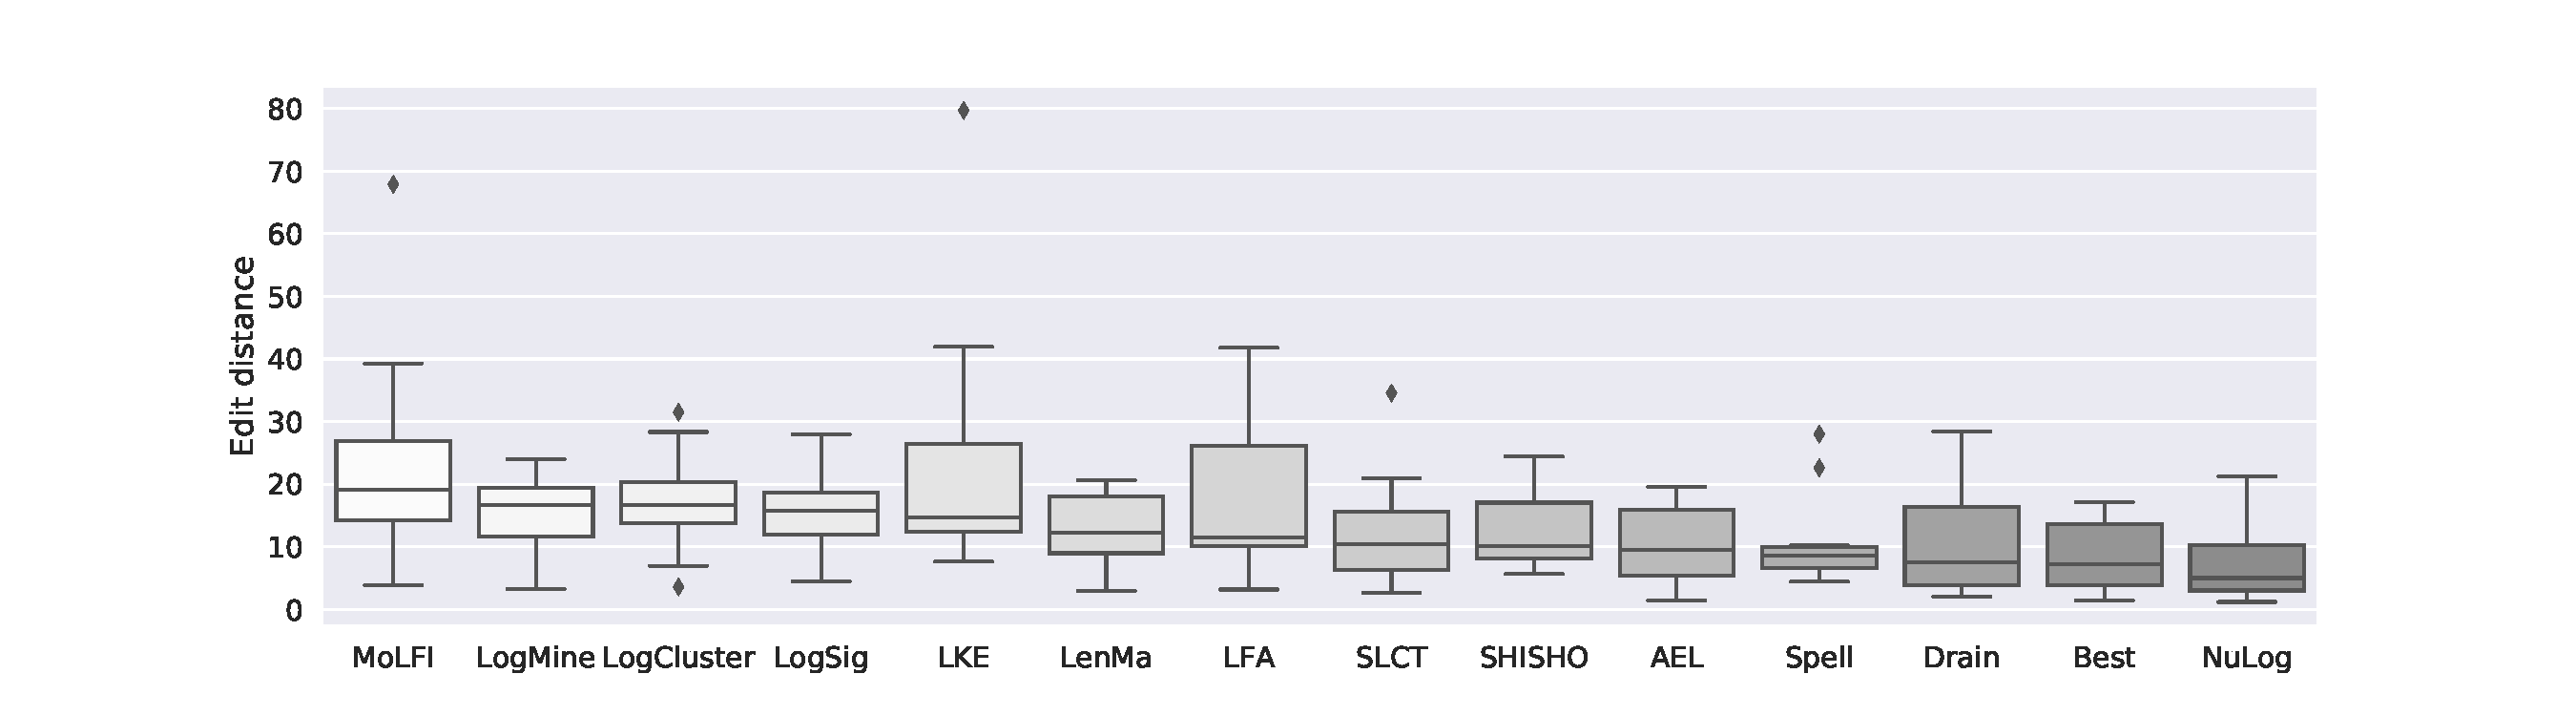
\includegraphics[width=1.0\textwidth]{gfx/chap4/robustness_ed.pdf}}
\caption{Robustness evaluation of the edit distance of the log parsers.}
\label{robustness_ed}
\end{figure}

\newpage 

\section{From log representations to log anomaly detection}
The improvement in the log parsing has a large impact on the subsequent log anomaly detection task in the traditional pipeline for a log analysis~\cite{zhu2019tools}. As described above, the next step in the log anomaly detection pipeline is to obtain log vectors. In previous unsupervised approaches, the log vectors are obtained by one-hot encoding of the templates or combination of word vectors using, e.g., word2vec~\cite{mikolov2013distributed}. In NuLog, these log vectors were directly produced together with the parsed log template. 
\begin{figure}[!b]
\centerline{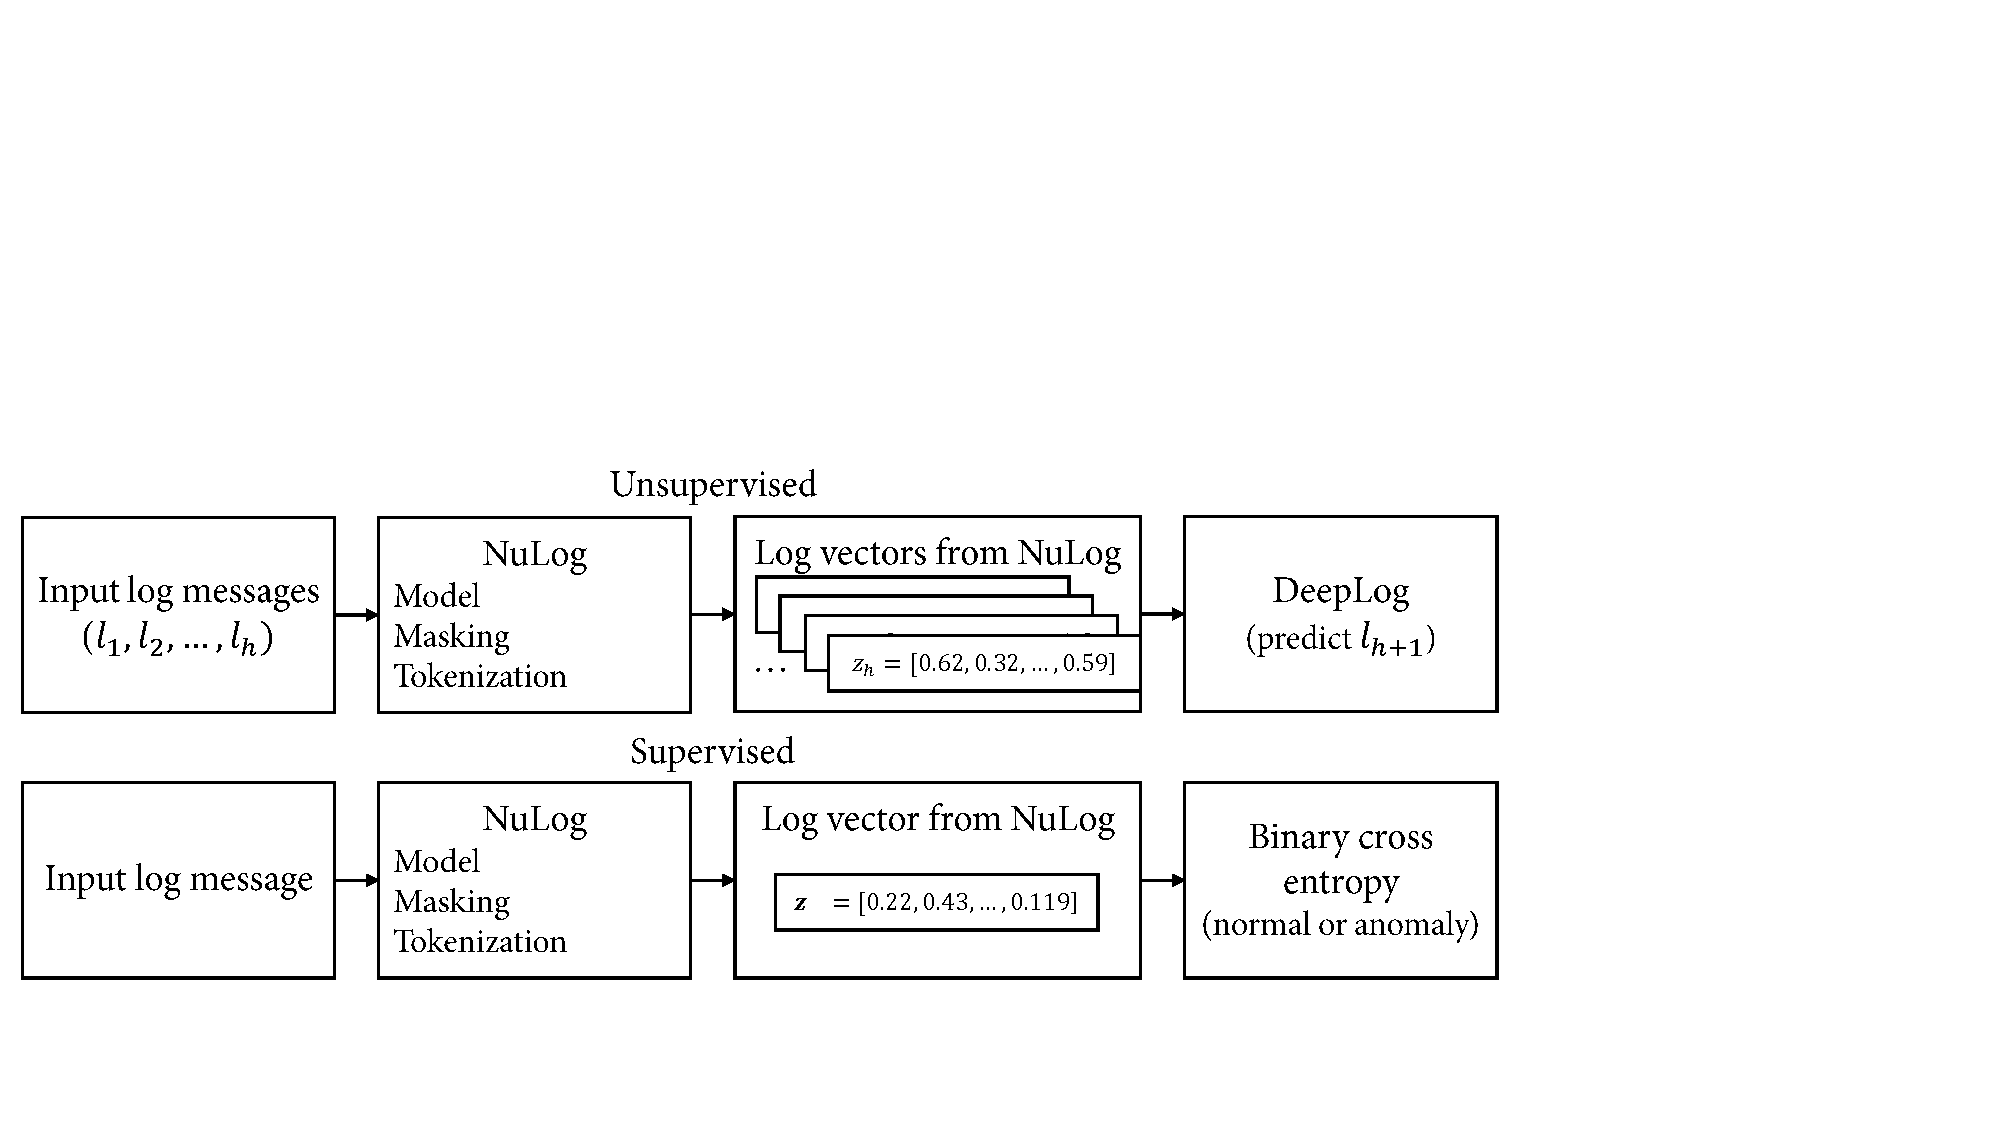
\includegraphics[width=1.0\textwidth]{gfx/chap5/nulogdeeplog.pdf}}
\caption{Unsupervised (top) and supervised (bottom) methods for downstream anomaly detection.}
\label{fig:downstream}
\end{figure}

We perform an additional analysis to compare the performances of (1) one-hot encoding of the templates, as they are utilized in the state-of-the-art log anomaly detection method, DeepLog~\cite{du2017deeplog}, (2) DeepLog with log vectors obtained from NuLog, instead of one-hot encoding, and (3) NuLog with an additional layer to perform supervised log anomaly detection.




We depict the unsupervised anomaly detection use case of NuLog in Figure~\ref{fig:downstream}. The log vectors from NuLog obtained from the ~\texttt{EMBEDDING} token are utilized by the modified DeepLog method instead of one-hot encoding to perform anomaly detection. DeepLog requires a sequence of $h$ log messages and learns to predict the next log message. If it successfully predicts the next log message, the message is classified as normal; otherwise, it is classified as an anomaly. 

In the supervised case, we learn the log message embeddings in a supervised manner. First, NuLog is trained on the parsing task. Second, we replace the last softmax layer by a linear layer, which maps the \texttt{EMBEDDING} vector to 0 or 1 (normal or anomaly), i.e., optimizes the model's parameters, as well as the log representations (the \texttt{EMBEDDING} vector) to perform binary classification. 


\begin{table}[htbp]
\centering
\caption{Scores for the anomaly detection use cases.}
\begin{tabular}{l|cc}
\hline
Method                     & \begin{tabular}[c]{@{}c@{}}BGL 10\%\\ 80\%-20\% train-test\end{tabular} & \begin{tabular}[c]{@{}c@{}}BGL 100\%\\ 80\%-20\% train-test\end{tabular} \\ \hline
DeepLog                    & 0.24                                                                    & 0.18                                                                     \\
DeepLog with NuLog vectors & 0.99                                                                    & 0.28                                                                     \\
Supervised NuLog            & 0.99                                                                    & 0.98                                                                     \\ \hline
\end{tabular}
\label{tab:nulogdeeplogsupervisedunsupervised}
\end{table}


Table~\ref{tab:nulogdeeplogsupervisedunsupervised} shows the results of the analysis. The vectors obtained from NuLog from the parsing task provided a higher performance in the anomaly detection than that of DeepLog. However, a large gap to the supervised learning scenario exists, where log vectors are learned using the available labels.

\begin{figure}[!b]
\centerline{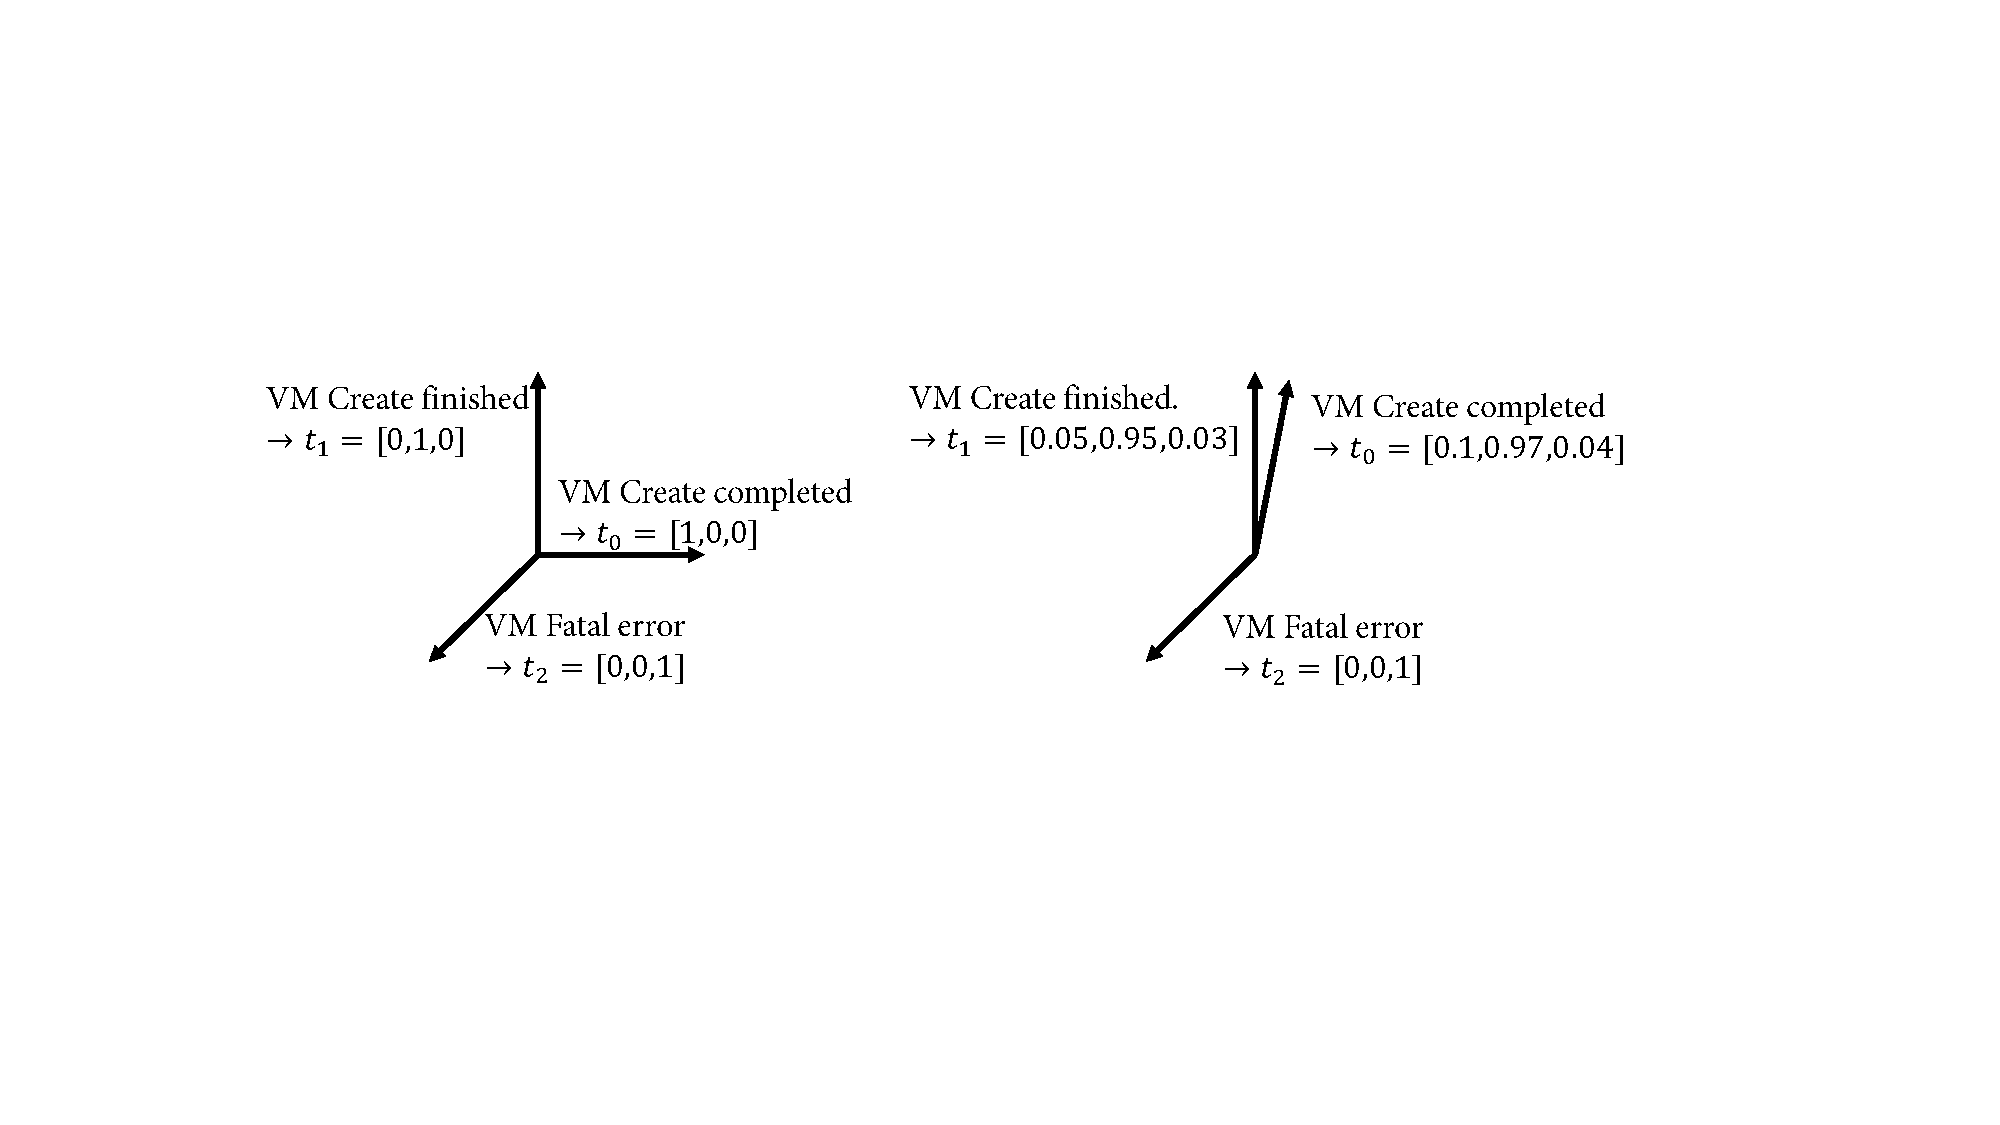
\includegraphics[width=1.0\textwidth]{gfx/chap5/orthogonallogvectors.pdf}}
\caption{Log vectors of three log messages, represented with one-hot encoding (indices, left) and desired representation (right).}
\label{fig:logrepresentations}
\end{figure}

The provision of better log vector representations increases the performances in the anomaly detection tasks. To show the importance of the log representations, we provide an example in Figure~\ref{fig:logrepresentations}. We illustrate three log messages when they are represented with one-hot encoding. The vectors are orthogonal and do not have similarity in-between. Therefore, when a new log message is observed, the model will recognize it as an anomaly, not similar to the learned log messages. This scenario of imperfect representations occurs also when word vectors pretrained on other domain are used. In an ideal case, "VM create finished" and "VM create completed" should be represented closely in the space, while "VM fatal error" should be distant from them. The normal samples should have compact representations, i.e., close distances in the representational space, while anomalies should be distant.

This, in the ultimate case, is shown with the supervised learning scenario of NuLog. When each log message is labeled, the method can identify compositions of words that signal normal and anomaly system states. Furthermore, it utilizes the semantic meaning of the log message to create better log vectors that are robust and produce accurate predictions even on unseen log messages. However, the provision of labeled data from specific systems in production is often prohibitive costly.


\begin{table*}[!t]
% \resizebox{1.0\textwidth}{!}{%
\centering
\begin{tabular}{l|l|c}
\hline
\textbf{Log message (log template $T$ in bold)} & \textbf{Class} & \textbf{Index}  \\ \hline
\textbf{total of} 77 \textbf{ddr error(s) detected and corrected}& normal & $x_0$    \\
\textbf{instruction cache parity error corrected} &normal & $x_1$    \\
\textbf{floating point unavailable interrupt}                             & anomaly       & $x_2$                 \\
\textbf{critical input interrupt (unit=}0x0b \textbf{bit}=0x06\textbf{)} &normal & $x_3$  \\ \hline
\end{tabular}
% }
\caption{Examples of log messages.}
\label{tab:logmessagestemplates}
\end{table*}

Supervised learning can be related to detection of anomalies in the log data by operators. They often analyze the semantic information from the logs and decide whether the message represents a severe system threat or failure. This semantic information is narrow and domain-specific. For example, in Table ~\ref{tab:logmessagestemplates}, $x_2$ and $x_3$ contain similar semantic meanings when observed without domain-specific knowledge. Therefore, both of them would be classified in the same class. However, if observed by a domain-expert knowing that a "floating point" interruption is considerably more severe than an "input" interruption, it would be able to recognize them correctly.

In the following sections of this chapter, we present a method, which addresses these challenges, and bridges the gap in effectiveness from unsupervised to supervised log anomaly detection.


\newpage 

\begin{figure}[!htbp]
\centerline{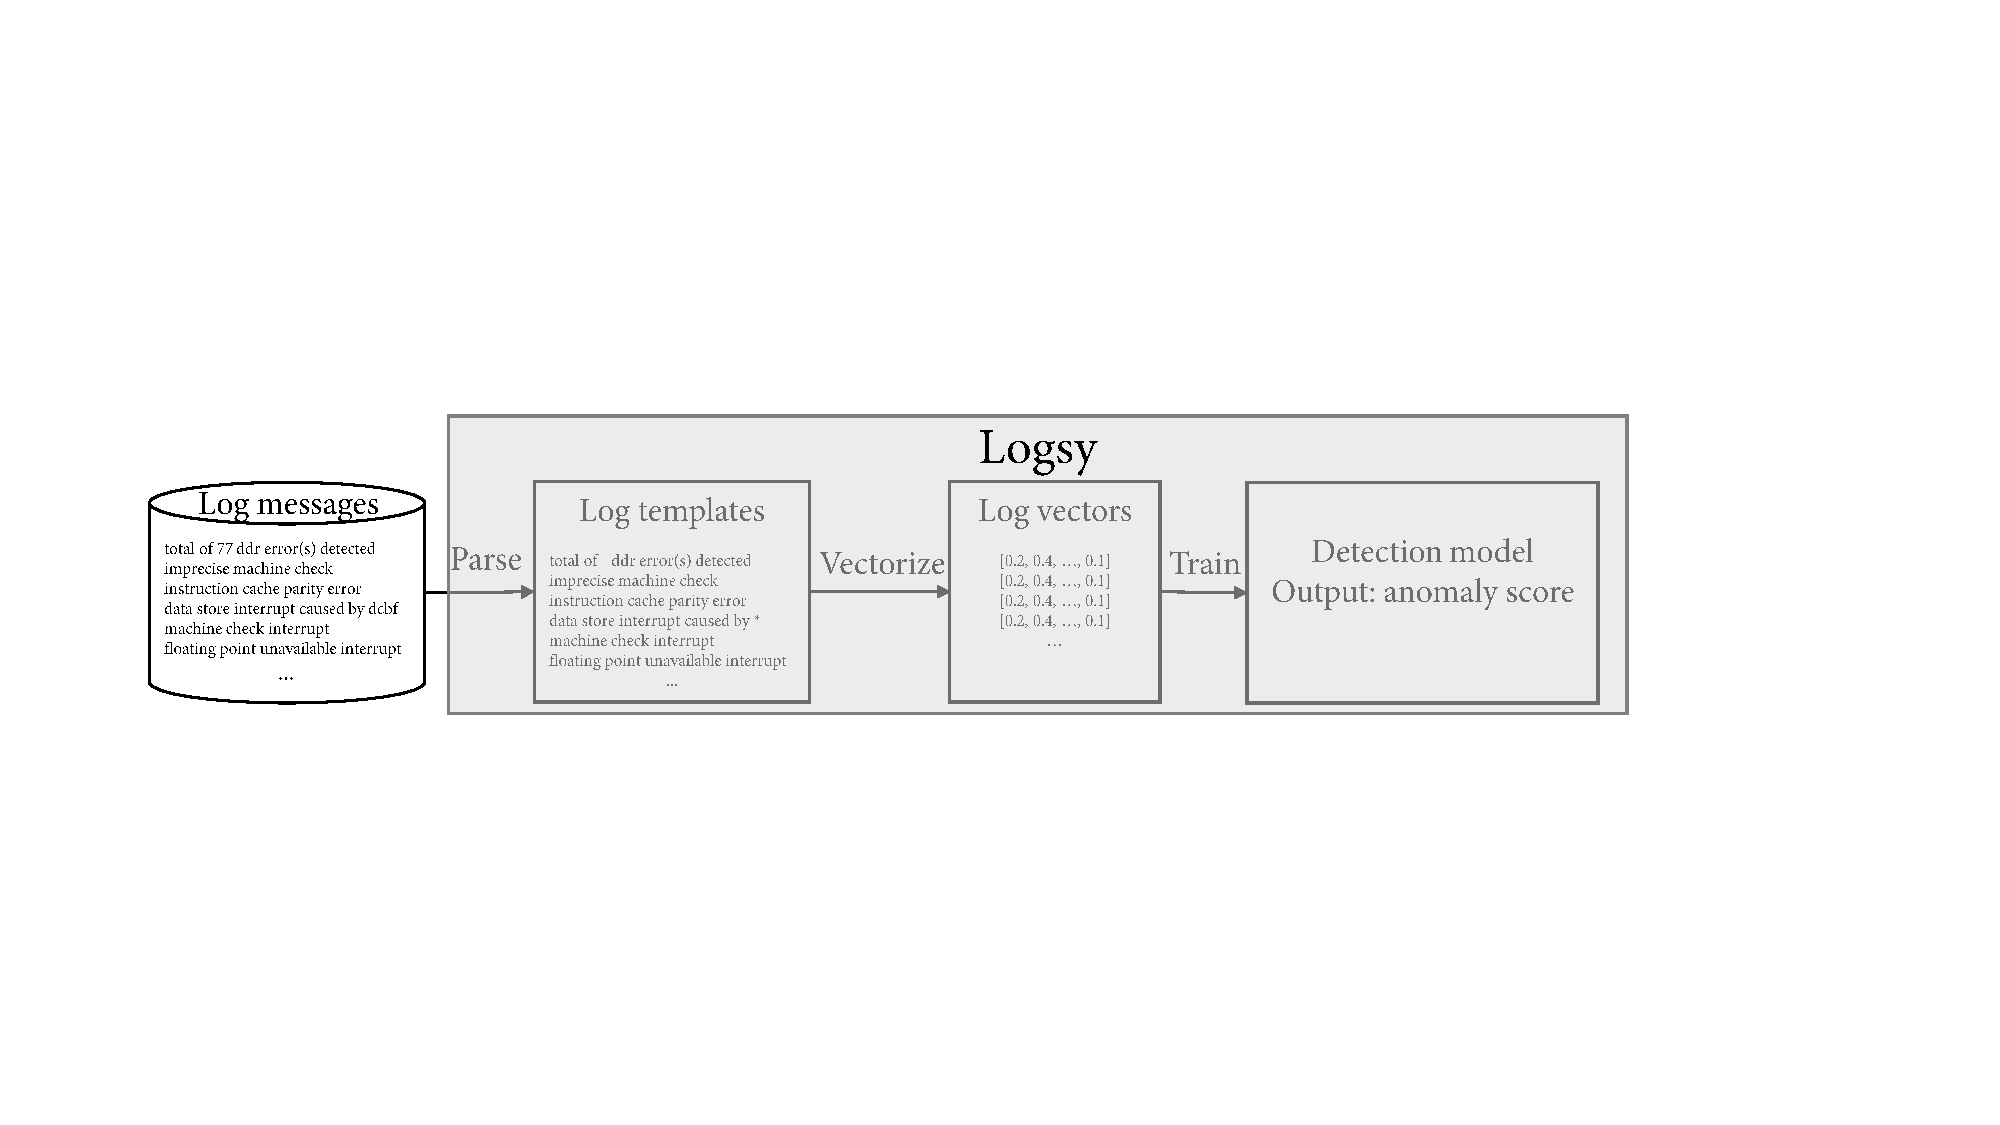
\includegraphics[width=1.0\textwidth]{gfx/chap5/logsypipeline.pdf}}
\caption{Logsy replacing the traditional pipeline of log anomaly detection.}
\label{fig:logsypipeline}
\end{figure}

\section{Log anomaly detection}
The normal log messages ideally should have vector representations with small distances between each other, e.g., concentrated within a tight sphere~\cite{ruff2019deep}. In this section, we present an anomaly detection method denoted as Logsy, which directly addresses the challenge of obtaining compact numerical log vectors. We train a neural network to learn log vectors to separate the normal log data from the system of interest (target system) and log messages from auxiliary log datasets from other systems, easily accessible through the internet. The concept of such a classification approach to anomaly detection is that the auxiliary dataset helps learn a more accurate representation of the normal data while regularizing against over-fitting. This leads to a better generalization for unseen logs. For example, for a target system of interest $T$ where anomaly detection needs to be performed, as auxiliary data, one or more datasets from an open-source log repository could be employed (~\cite{oliner2007supercomputers}). To model the data, we reuse the same transformer architecture as in NuLog. Additionally, we propose a hyperspherical, instead of the traditional hyperplane classification decision boundary, learning objective, to learn compact log vector representations of the normal log messages. This enforces the normal samples to have concentrated (compact) vector representations around the center of a hypersphere. Small distances from the center correspond to normal samples, while large distances correspond to anomalies. The method enables a direct log-to-vector transformation, which can be used to improve the performances of previous related methods.

In this regard, we shift from the traditional log anomaly detection pipeline (Figure~\ref{fig:logsypipeline}). With Logsy, we learn the anomaly score end-to-end from raw log messages. The method does not depend on log parsing and does not utilize a module for obtaining log vectors. The log parsing and log vectorization in Logsy are learned implicitly during the training procedure. 


\subsection{Importance of the auxiliary data}
To elucidate the importance of using the auxiliary data, we relate the anomaly detection task to 
the task of density level set estimation~\cite{tsybakov1997nonparametric}. Steinwart et al.~\cite{steinwart2005classification} stated that this can be interpreted as a binary classification between the normal and anomalous distributions and that the prior on the anomalous distribution is essential for an improved detection. Thus, if we provide information to the model regarding the distribution of the anomalous data, it will increase its performance. For example, we may interpret the class assumption in semi-supervised anomaly detection that a small number of anomaly data points are available and labeled as such prior knowledge or bias~\cite{ruff2019deep}. Moreover, specific types of data can have inherent properties, which enables more informed prior assumptions such as the word representations in texts~\cite{bengio2013representation}, where it is assumed that each word meaning depends on its context.

We assume that drawing realistic samples from some auxiliary easy-access corpus of log data can be considerably more informative for an added description of normal data and anomalies compared to the sampling noise. These samples are replacements for real anomalies used, e.g., in semi-supervised learning approaches.

\section{\textit{Logsy:} Classification-based anomaly detection on logs}
In this section, we explain the proposed method in detail. We describe the data preprocessing, neural network model, log vector representations, and their utilization in the modified objective function for anomaly detection.

To formally define the task, we consider $\mathcal{D}=\{(\mathbf{x_1}, y_1), \dots, (\mathbf{x_n}, y_n)\}$ as training logs from the system of interest where $\mathbf{x_i}$ is a log message whose tokens are represented in $d-dimensional$ space (the log message is represented by $d\times \vert r \vert$ matrix, where $\vert r \vert$ is the maximum number of tokens in all log messages) and $y_i=0; 1 < i \leq n$, assuming that the data in the system of interest are composed mostly of normal samples. $\mathcal{A}=\{(\mathbf{x_n}, y_{n}),\dots, (\mathbf{x_{n+m}}, y_{n+m})\}$, where $m$ is the size of the auxiliary data and $y_i={1}; n < i \leq n+m$. $\phi(\mathbf{x_i}, y_i, \theta): \mathbb{R}^{d \times |r_i|} \rightarrow \mathbb{R}^p \rightarrow [0, a], a \in \mathbb{R}$ is a function represented by a neural network, which maps the input log message token embeddings to vector representations in $\mathbb{R}^p$ (log vectors), and then to an anomaly score. The task is to learn the parameters $\theta$, and then, for each incoming instance in the prediction phase $\mathcal{D}_t=\{(\mathbf{x_1^t}), (\mathbf{x_2^t}),\dots, (\mathbf{x_j^t}), \dots\}$, predict whether it is anomalous or normal based on the anomaly scores, where $t$ indicates the test sample.

\begin{figure}[!b]
\centering
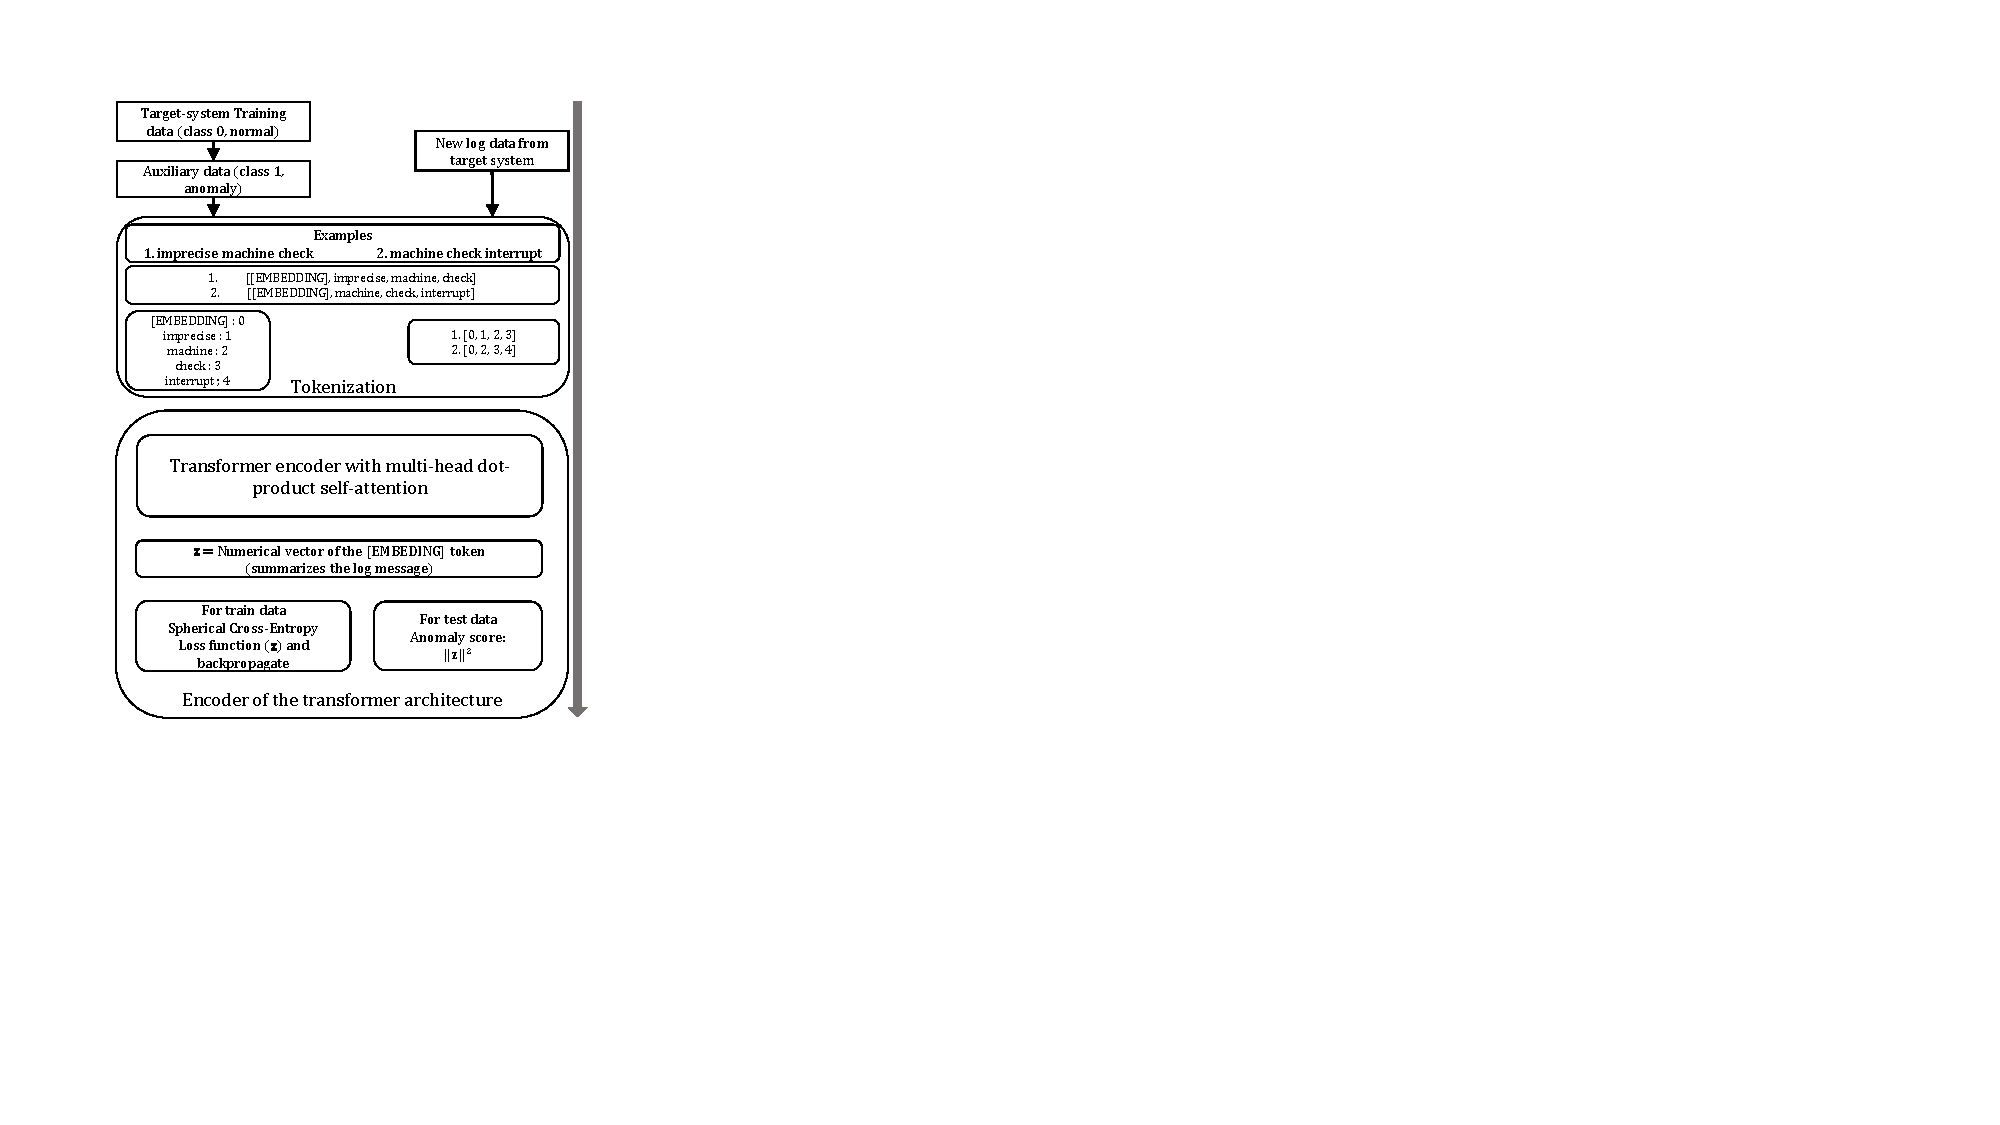
\includegraphics[width=0.8\textwidth]{gfx/chap4/model_loganomalydetection.pdf}
\caption{Overview of the architecture and component details of Logsy.}
\label{overviewmethod}
\end{figure}

\subsection{Logsy}
The method is composed of two main parts, the tokenization of the log messages and neural network model.

\textbf{Tokenization.} The tokenization transforms the raw log messages into a sequence of tokens, as shown in Figure~\ref{overviewmethod}. The same tokenization module as in NuLog is used. In addition, in the tokenization module, we perform cleaning of the log messages. For this purpose, we utilize the standard text preprocessing library NLTK~\cite{loper2002nltk}. The message is initially filtered for HTTP and system path endpoints (e.g., /p/gb2/stella/RAPTOR/). Every capital letter is converted to the lowercase letter. All ASCII special characters are removed. The log message is split into word tokens. We remove every token that contains numerical characters, as they often represent variables in the log message and are not informative. Additionally, we remove the most commonly used English words that are in the stop word dictionary of NLTK (e.g., the and is). Similar to the case of NuLog, to the front of the tokenized log message, a special \texttt{EMBEDDING} token is added. In the model, the \texttt{EMBEDDING} token attends over all original tokens from the sample, which enables the model to summarize the context of the log message in the vector representation. All tokens from every log message form a dictionary $\mathbb{V}$ with a size of $|\mathbb{V}|$, where each word is represented with an integer label $i \in {0, 1, \dots,|\mathbb{V}|-1}$. An advantage of Logsy over previous log anomaly detection approaches is that it does not depend on log parsers as a preprocessing step (only cleaning). We consider the tokenized log message as a direct input to the model. As an advantage, no loss of information from the log message exists, owing to the imperfections in the log parsing methods.

\textbf{Model}. Logsy has two operation modes, offline and online. During the offline phase, log messages are used to tune all model parameters through back-propagation and optimal hyperparameters are selected. During the online phase, every log message is passed forward through the saved model. This generates the respective log vector representation $\mathbf{z}$ and anomaly score for each message.

The core model architecture is the Transformer encoder, similar to NuLog. As a detailed description of the transformer encoder was already presented in~\autoref{NuLog}, we describe only the major parts.
The model applies two operations on the input tokens, token vectorization (word embeddings) and positional encoding. The subsequent structure is the encoder of the transformer~\cite{vaswani2017attention} module with a multi-head self-attention, which uses the result of these operations as an input. 
At the output of the encoder, the transformed vector representation from the initial tokens exists. The \texttt{EMBEDDING} token has its transformed representation $\mathbf{z}$, which is used as a final log vector representation.
The final element of the model consists of a single linear layer. It receives the vector $\mathbf{z}$ from the \texttt{EMBEDDING} token and uses it for optimizing the model. Based on the loss function, gradients are back-propagated to tune the parameters of the model. 

\subsection{Objective function}
To ensure learning of the intrinsic differences between normal and anomaly log samples, we propose a spherical loss function. It is designed to integrate the previously mentioned assumption that normal data are often concentrated, with small distances between the normal samples, while also learning properties to distinct from anomalous samples. This is carried out by employing a radial classification loss, which enforces a compact hyperspherical decision region for the normal samples.

To derive the loss, we start with the standard binary cross entropy. $\mathcal{D}=\{(\mathbf{x_1}, y_1), \dots, (\mathbf{x_{n+m}}, y_{n+m})\}$ is the concatenation of the training logs from the system of interest and auxiliary data with $\mathbf{x_i} \in \mathbb{R}^{d\times|r_i|}$, where $|r_i|$ is the number of tokens in the log message and each token is a vector represented in $d-dimensional$ space. $y_i \in \{0,1\}$; $y_i=0$ denotes normal samples (target system), while $y_i=1$ denotes an anomaly (auxiliary data). $\phi(\mathbf{x_i}, \theta): \mathbb{R}^d \rightarrow \mathbb{R}^p$ is our encoder architecture, which maps the $|x_i|$ word embeddings form the log message to a $p-dimensional$ vector. $l:\mathbb{R}^p \rightarrow [0,1]$ is a function that maps the output to an anomaly score. Using $\phi(\mathbf{x_i}, \theta)$ and $l(\cdot)$, the standard binary cross-entropy loss can be expressed by

\begin{equation}
    - \frac{1}{n}\sum_{i=1}^{n}(1-y_i)\log l(\phi(\mathbf{x_i}; \theta)) + y_i\log (1-l(\phi(\mathbf{x_i}; \theta))).
\end{equation}\label{bce}

For the standard classifier function, the $p-dimensional$ representation is transformed through a linear layer followed by the sigmoid activation function,

\begin{equation}\begin{aligned}
    - \frac{1}{n}\sum_{i=1}^{n}(1-y_i)\log((1+\exp(-\mathbf{w}^T \phi(\mathbf{x_i}, \theta)))^{-1}) \\
    +  y_i\log(1-(1+\exp(-\mathbf{w}^T \phi(\mathbf{x_i}, \theta)))^{-1})\end{aligned}.
\end{equation}\label{bcesigmoid}

In the standard binary classifier with the sigmoid function, the decision boundary is half-space, as depicted in gray in Figure~\ref{hyperplane}. The representation of the log messages is not guaranteed to be compact in this case. It is very likely that the normal samples are scattered throughout the space with varying potentially very large distances between them. To enforce compactness of the representations of the log messages, we utilize the Gaussian radial basis function, $l(\cdot)$,

\begin{equation}
    l(\mathbf{z})= \exp(-\Vert \mathbf{z} \Vert ^2).
\end{equation}

By replacing the function into the loss function, we obtain the hyperspherical classifier,
\begin{equation}\begin{aligned}
    - \frac{1}{n}\sum_{i=1}^{n}(1-y_i)\log(\exp(-\Vert \phi(\mathbf{x_i}; \theta) \Vert ^2)) \\
    +  y_i\log(1-\exp(-\Vert \phi(\mathbf{x_i}; \theta) \Vert ^2)) \\
    =  \frac{1}{n}\sum_{i=1}^{n}(1-y_i)\Vert \phi(\mathbf{x_i}; \theta) \Vert ^2 \\
    -  y_i\log(1-\exp(-\Vert \phi(\mathbf{x_i}; \theta) \Vert ^2)).\end{aligned}
\label{hce}
\end{equation}.


This ensures compactness of the normal samples, which are enforced to be around the center of a sphere $\mathbf{c}=\mathbf{0}$. For normal samples, i.e., $y_i=0$, the loss function minimizes the distance to $\mathbf{c}$. This leads to low values for the left term in Equation~\ref{hce}. In contrast, the right term of the loss function favors large distances for the anomalous samples. As shown in Figure~\ref{hypersphere}, the radial basis function has a spherical (circle in 2D) decision boundary, located between the gray and black areas. The center of the sphere $c$ could be any constant value, which is not relevant during the optimization.


\begin{figure}[!t]
\minipage{0.35\columnwidth}
  
\includegraphics[width=\linewidth]{gfx/chap4/hyperplane.pdf}
  \caption{Hyperplane classifier with sigmoid.}\label{hyperplane}
\endminipage\hfill
\minipage{0.45\columnwidth}
  
\includegraphics[width=\linewidth]{gfx/chap4/hypersphere.pdf}
  \caption{Hypersphere classifier using the radial function instead of sigmoid.}\label{hypersphere}
\endminipage

\end{figure}

However, for such spherical classifiers~\cite{ruff2019deep}, the model may be prone to learn trivial solutions by mapping the inputs to output a constant vector, $c$. However, the proposed loss function will not find the trivial solution because of the second term in the equation, which represents the auxiliary data or anomalies. To formally demonstrate this statement, we consider $\phi(\cdot)$ as an encoder network, which maps every log message to $\mathbf{c}$ (trivial solution). Thus, $\phi(\cdot)=\mathbf{0}$. In this case, the second term in Equation~\ref{hce} for $y_i=1$ will be infinity or very large value, which acts as a regularizer and prevents learning $\mathbf{c}$ as a trivial vector representation,

\begin{equation}\begin{aligned}
    -\log(1-\exp(-\Vert \mathbf{0} \Vert ^2))= -log(\mathbf{0}).
    \end{aligned}
\end{equation}\label{hcedecomposed}

\subsection{Anomaly score and detection of anomalies}
Considering that the assumption of the objective function enforces compact, close to the center of the sphere $\mathbf{c}=\mathbf{0}$, representations, we define our anomaly score as the distance of the log vectors (obtained from the \texttt{EMBEDDING} token) to the center $\textbf{c}$ of the hypersphere,

\begin{equation}
    A(\mathbf{x_i}) = \Vert \phi(\mathbf{x_i}; \theta) \Vert ^2.
\end{equation}

We attribute low anomaly scores $A(\mathbf{x_i})$ to normal log messages, while large scores to anomalies. To decide whether the sample is anomalous or normal, we use a threshold $\mathcal{E}$. If the anomaly score $A(\mathbf{x_i}) > \mathcal{E}$, the sample is an anomaly; otherwise, we consider it as normal. This concludes the explanation of the method. We describe two properties of the model below.


\subsection{Learning with an additional expert input}
Most computer systems are, to some extent, supervised and operated by an administrator. Over time, the administrator can manually inspect a small portion of the events and provide labels.
As an additional option, Logsy allows incorporation of such labels from the target system. The second term in Equation~\ref{hce}, used for the auxiliary data, could be also utilized for the inclusion of operator-labeled samples. This enables the addition of even more realistic, but costly anomaly samples, which help learn the anomaly distribution and improve the performance. The labeled samples can be added together with the auxiliary data and the model needs to be retrained or the following procedure should be utilized:
\begin{enumerate}
    \item Train the model with the auxiliary data.
    \item Replace the auxiliary data with the labeled samples.
    \item Continue the training of the model only with the labeled sample until convergence.
\end{enumerate}

The replacement of the auxiliary data with the labeled samples allows the model to only fine-tune its parameters in a few epochs. This preserves the already learned information from the larger auxiliary dataset as a bias to the fine-tuning procedure. In the experiments, we show that the inclusion of a small portion of labeled samples improves the performance of the model.



\begin{figure}[!b]
\centering
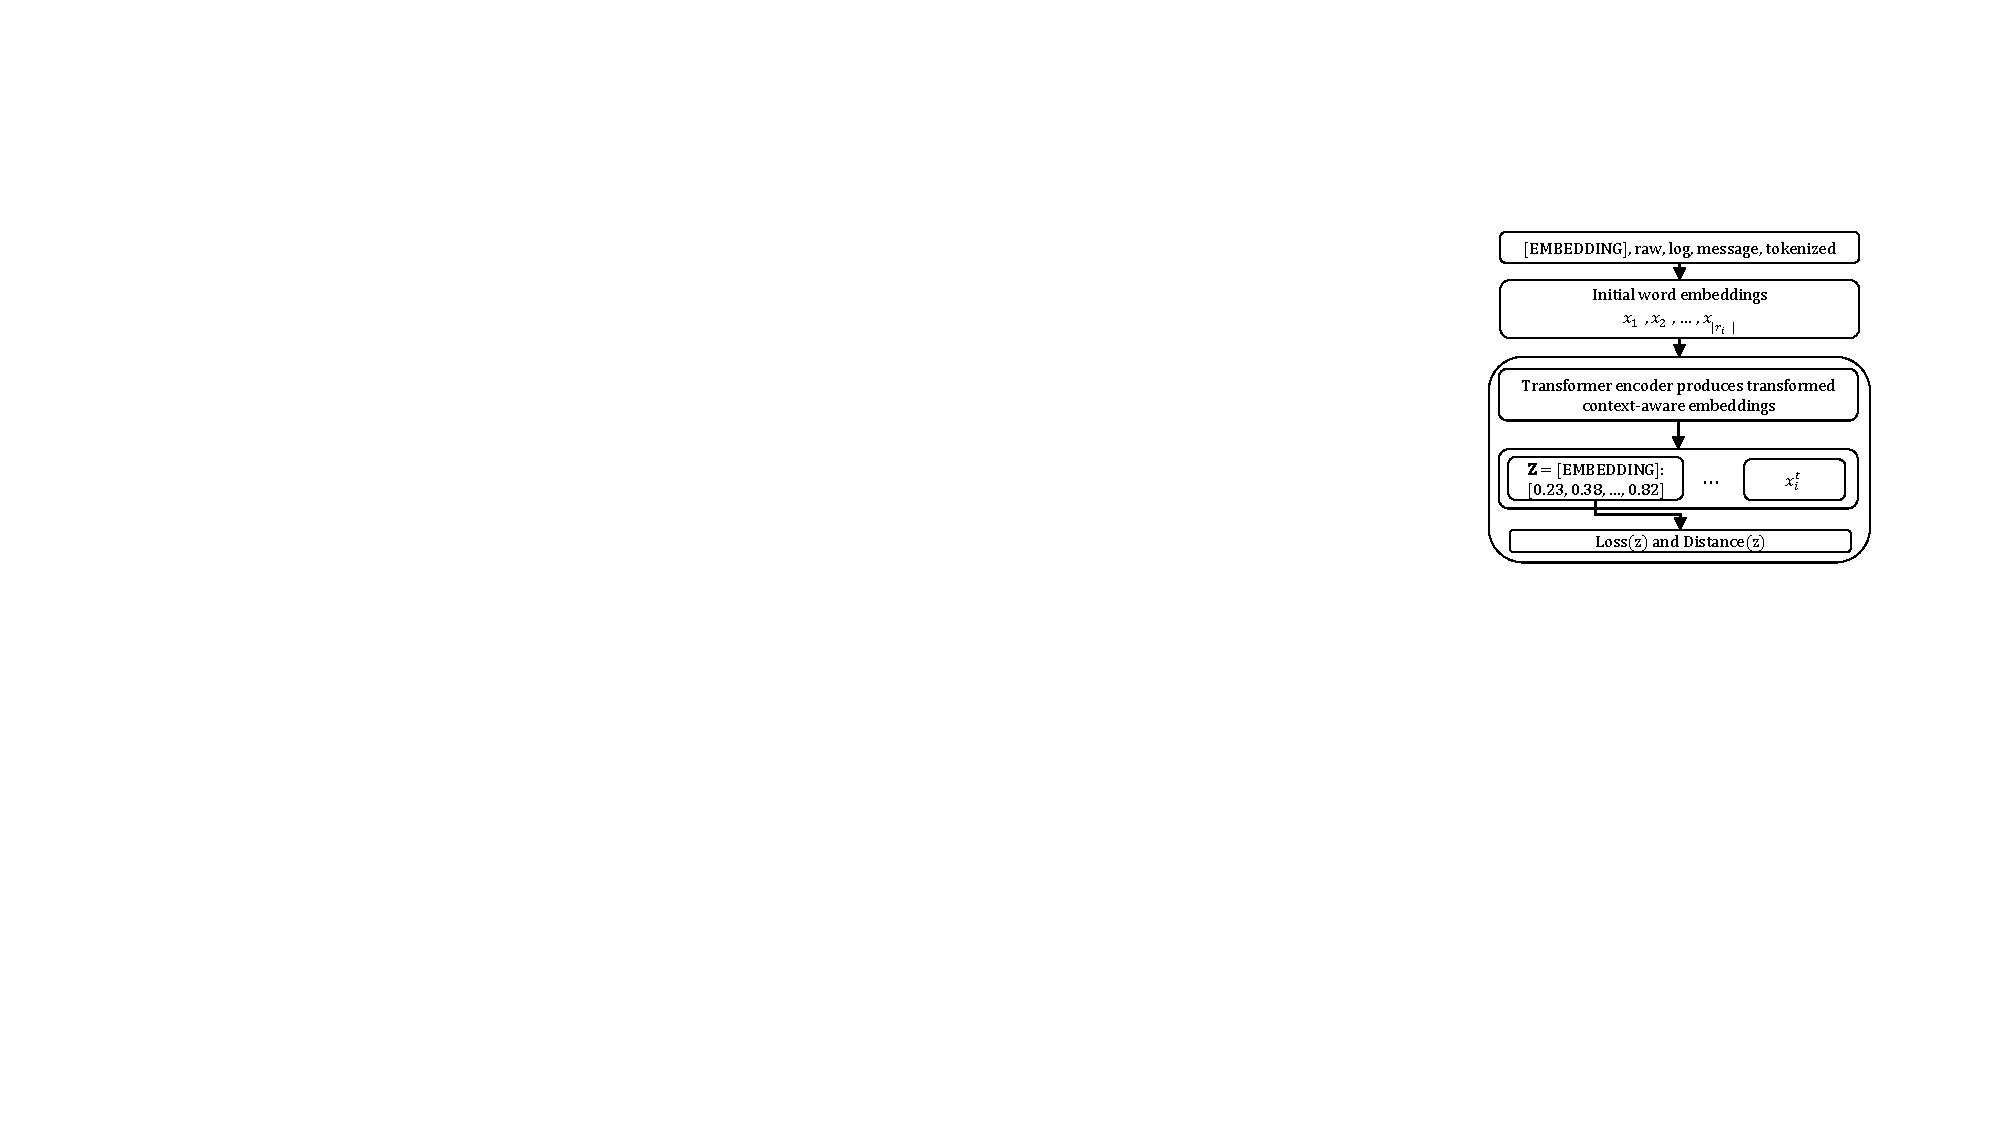
\includegraphics[width=0.7\textwidth]{gfx/chap5/gettingembeddings.pdf}
\caption{Provision of the log vector embedding using the special 'EMBEDDING' token that summarizes the context of the log message.}
\label{fig:gettingembeddings}
\end{figure}


\begin{figure}[!t]
    \centering
    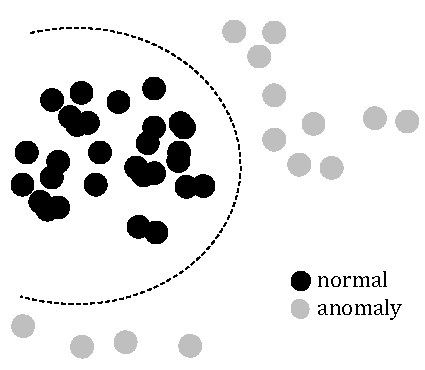
\includegraphics[width=0.6\columnwidth]{gfx/chap4/embeddingsinspace.pdf}
    \caption{Ideal distribution of the log vector representations in space.}
    \label{fig:lowdimensions}
\end{figure}


\subsection{Vector representations of the logs}\label{vectorrepresentations}
Logsy can also be utilized to obtain numerical log representations as they are used in the traditional log anomaly detection pipeline. These representations, as described above, are used by the objective function and to obtain anomaly score in Logsy, but could be also used to replace other less powerful representations, e.g., term-frequency inverse document frequency (TF-IDF) in previous log-based anomaly detection methods such as the PCA ~\cite{xu2009detecting}), to enhance their anomaly detection. 

In Figure~\ref{fig:gettingembeddings}, we illustrate the process of obtaining the log embeddings. The transformer encoder transforms each of the vectors of the input tokens $x_1, x_2, \dots, x_{|r_i|}$ to an abstract representation $x_1^t, x_2^t, \dots, x_{|r_i|}^t$. As only the vector of the first \texttt{EMBEDDING} token is used for optimizing the loss function, it summarizes the context of the log message. In Figure~\ref{fig:lowdimensions}, we illustrate a lower-dimensional plot of the ideal log representations. A decision boundary (dashed line) can be drawn to optimally separate the classes. We demonstrate such behavior in the evaluation section on real data with Logsy, where we show the normal and abnormal sample distributions in a low-dimensional space.

\newpage

\section{Evaluation}
We perform various experiments to quantify the performance of Logsy. We compare the method against two publicly available baselines, DeepLog and PCA, on three real-world HPC log datasets. We describe the main properties of the datasets and experimental setup and present the results. We empirically and qualitatively evaluate the log vector representations from Logsy. We utilized them in the PCA method, which provided an improved performance.



\begin{table*}[!b]
\resizebox{\columnwidth}{!}{%
\begin{tabular}{c|c|c|c|c|c|c|c}
\hline
\textbf{System} & \textbf{Vendor} & \textbf{\#Processors} & \textbf{Days} & \textbf{\#Messages} & \textbf{Data Size (GB)} & \textbf{\#Anomalies} & \textbf{\#Anomalies (5m)} \\ \hline
Blue Gene/L     & IBM             & 131072                & 215           & 4747963             & 1207                    & 348460               & 348460                 \\
Thunderbird     & Dell            & 9024                  & 244           & 211212192           & 27367                   & 3248239              & 226287                 \\
Spirit          & HP              & 1028                  & 558           & 272298969           & 30289                   & 172816564            & 764890 \\\hline               
\end{tabular}
}
\caption{Target datasets.}
    \label{datasets}
\end{table*}




\subsection{Experimental setup}
We select three open real-world datasets from HPC systems for the evaluation as target systems, Blue Gene/L (BGL), Spirit, and Thunderbird~\cite{oliner2007supercomputers}. Table~\ref{datasets} summarizes the main characteristics of the datasets. They share an important characteristic associated with the appearance of numerous new log messages in the timeline of the data, i.e., the systems change over time. Furthermore, as an additional dataset for enriching the auxiliary data in all experiments, we use the HPC RAS log dataset~\cite{zheng2011co}. Owing to the absence of labels, this dataset cannot be used for evaluation purposes; it cannot be a target dataset. 

For each target dataset, as auxiliary data to represent the anomaly class, we use logs from the remaining datasets. Notably, the target vs. auxiliary splits ensure that no leak of information from the target system into the auxiliary data exists. The auxiliary logs consist only of easily accessible logs from other systems through the internet. 
The nonanomalous samples from the target system are the target dataset. For example, when Blue Gene/L is our system of interest (i.e., the target system), percentages of the negative samples of Thunderbird, Spirit, and RAS are used as an auxiliary dataset to represent the anomaly class. These auxiliary samples could be also error messages obtained from online code repositories (e.g., GitHub).
We perform anomaly detection on the test samples from the target dataset to determine the scores. The setup is illustrated in Figure~\ref{fig:datasplits}.


\begin{figure}[!htbp]
    \centering
    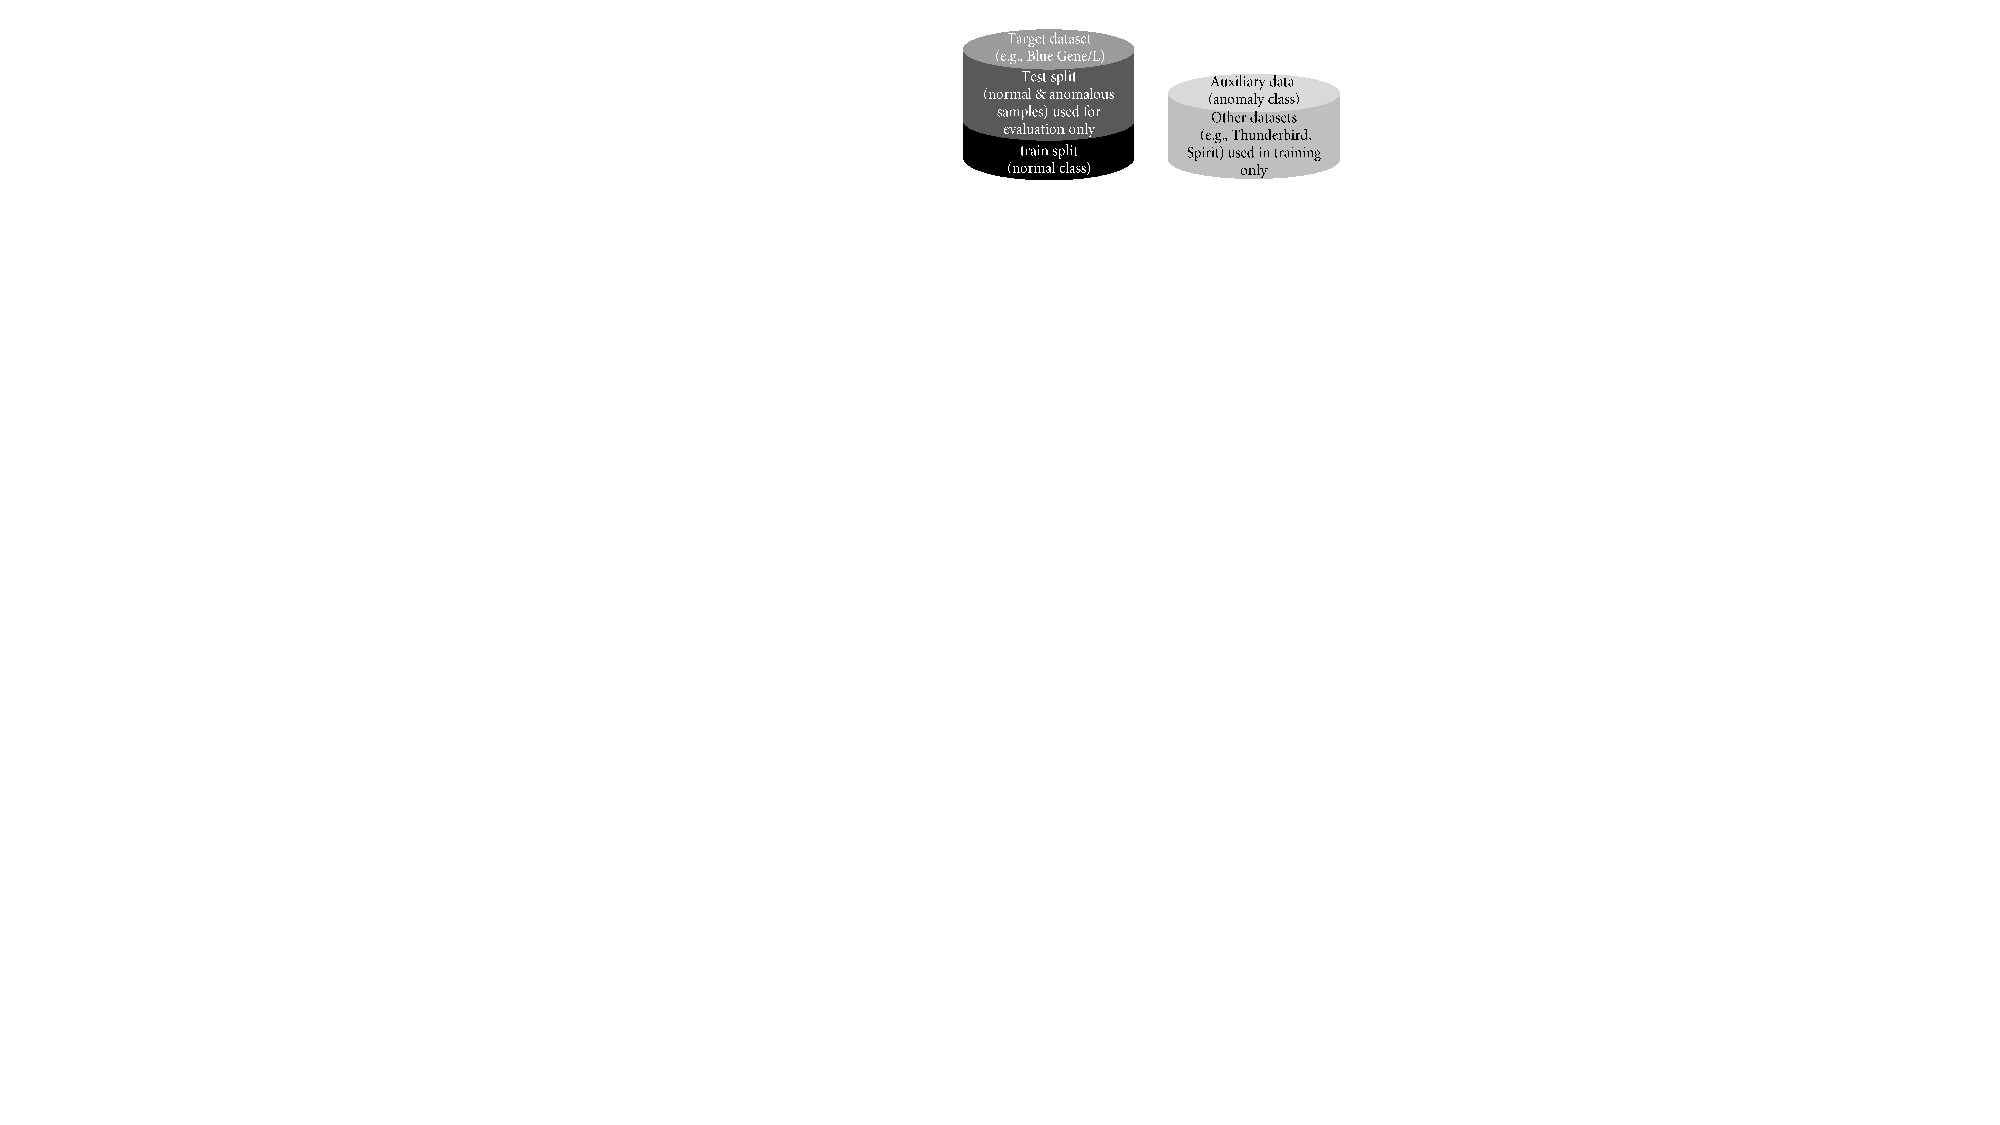
\includegraphics[width=0.7\columnwidth]{gfx/chap5/datasplits.pdf}
    \caption{Illustration of the target and auxiliary data split.}
    \label{fig:datasplits}
\end{figure}

Table~\ref{datasets} shows that Thunderbird and Spirit are quite large datasets of more than 200 million log messages. For a computation time reduction, we restrict the data size on the first 5 million log messages, sorted by timestamp. We ensure that the 5 million log lines preserve the properties of the dataset. Table~\ref{unqiuemessages} shows the number of unseen logs in the test data split. The Blue Gene/L dataset has less than 5 million messages; thus, we keep all of them. \#Anomalies (5m) shows the number of anomalous log messages in the 5 million messages. 



To evaluate the robustness and generalization of Logsy in detail, we carry out several experiments with different train--test splits on the target dataset. To ensure that the test data contain new log messages previously unseen in the training, we always split the data sorted by the timestamp of the log messages. We perform five different data splits to cover as many scenarios as possible: 10\% training -- 90\% test data, 20\% training -- 80\% test, 40\% training -- 60\% test, 60\% training -- 40\% test, and 80\% training -- 20\% test.

The number of unique log messages after the tokenization is presented in Table~\ref{unqiuemessages}. Every split contains unseen log messages in the test data, which do not exist in the train split. The evaluation of the method on such splits demonstrates the model generalization. The decrease in the size of the training data increases the number of novel log messages in the test split.

\begin{table}[!htbp]
\centering
\begin{tabular}{c|c|c|c|c|c|c}
\hline
{\textbf{System}} & \multicolumn{5}{c|}{\textbf{\begin{tabular}[c]{@{}c@{}}\#Unique log messages in \\ test and not present in train for every split\end{tabular}}} & {\textbf{\begin{tabular}[c]{@{}c@{}}\#Total unique\\ messages\end{tabular}}} \\ \cline{2-6}
                                 & \multicolumn{1}{l|}{10\%}     & \multicolumn{1}{l|}{20\%}     & \multicolumn{1}{l|}{40\%}     & \multicolumn{1}{l|}{60\%}     & 80\%    &                                                                                             \\ \hline
Blue Gene/L                      & 2679                          & 2621                          & 2256                          & 2231                          & 465     & 4486                                                                                        \\
Thunderbird                      & 334                           & 127                           & 71                            & 27                            & 12      & 3279                                                                                        \\
Spirit                           & 1091                          & 1028                          & 297                           & 129                           & 73      & 3441                                                                                        \\ \hline
\end{tabular}
\caption{Number of new log messages in the test in every train/test split.}
\label{unqiuemessages}
\end{table}

\subsection{Baselines}
We compare Logsy against two publicly available baseline methods, PCA~\cite{xu2009detecting} and Deeplog~\cite{du2017deeplog}. Industry related studies showed that LogAnomaly~\cite{meng2019loganomaly} has a state-of-the-art performance. However, it has no publicly available implementation. LogAnomaly provides an improvement compared to DeepLog with an F1 score of 0.03. The results of both methods are comparable. The parameters of these methods are tuned to produce their best F1 scores.

\subsection{Implementation details}
Every log message during the tokenization is truncated to a maximum of $\max(\vert r_i \vert)=50$ tokens. Logsy has two layers of the transformer encoder. The words are embedded with 16 neural units. The higher-level vector representations obtained with the transformer encoding have the same sizes. The size of the feed-forward network that uses the output of the multi-head self-attention mechanism is also 16, which provides the '[EMBEDDING]' vector with the same size. For the optimization procedure for every experiment, we use a dropout of 0.05, Adam optimizer with a learning rate of 0.0001, and weight decay of 0.001. We address the imbalanced number of normal versus anomaly samples by adding weights to the loss function for the two classes, 0.5 for the normal and 1.0 for the anomaly class. The models are trained until convergence and later evaluated on the respective test split.




\begin{figure*}[!t]
    \centering
    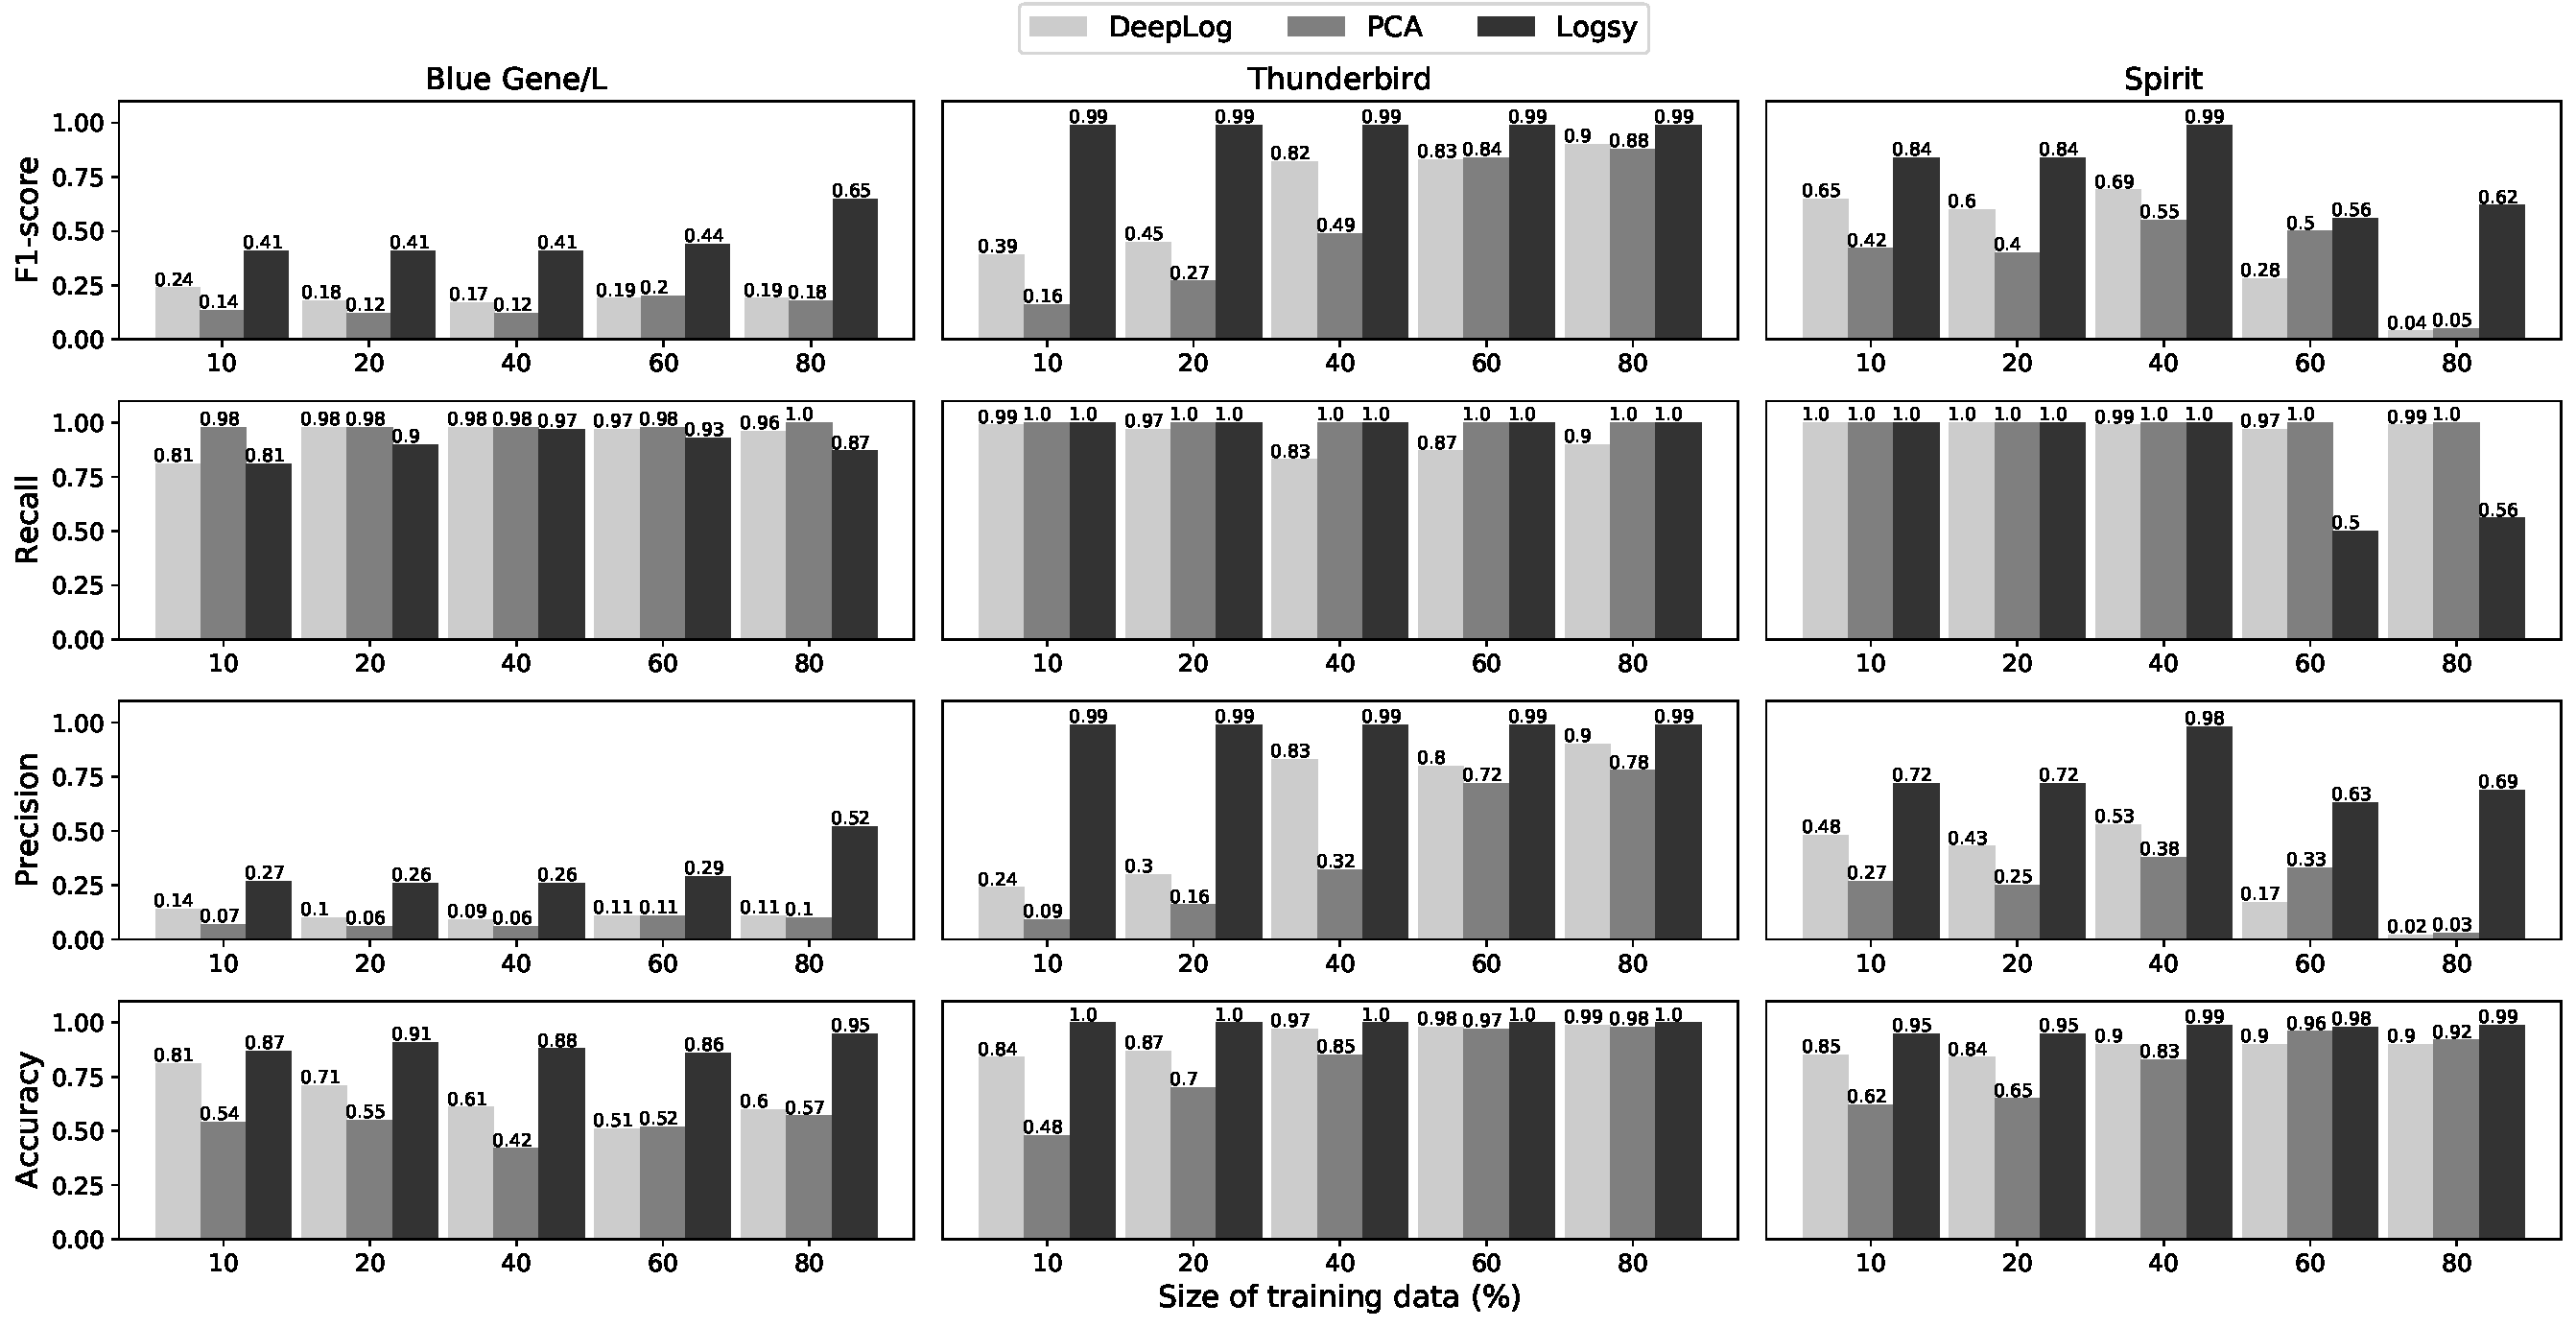
\includegraphics[width=1.0\textwidth]{gfx/chap4/results.pdf}
    \caption{Comparison of the evaluation scores against the two baselines DeepLog and PCA on three different datasets.}
    \label{fig:results}
\end{figure*}


\subsection{Results and discussion}
We show the overall performance of Logsy compared to the baselines in Figure~\ref{fig:results}. Generally, Logsy achieves the best scores, with an averaged F1 score in all splits of 0.448 on the Blue Gene/L dataset, 0.99 on the Thunderbird dataset, and 0.77 on the Spirit data. DeepLog and PCA have lower F1 scores in all performed experiments. The baselines have a very high recall, but low precision. This implies that they can find the anomalies. However, they will produce large numbers of FP predictions. 

Logsy preserves the high recall across the datasets and evaluation scenarios. In addition, it exhibits a large improvement in the precision scores, owing to the correct classification of new unseen log messages and reduction in the FP rate. For example, on the Blue Gene/L dataset, DeepLog and PCA exhibit 2--4 times lower precisions than that of Logsy. Overall, Logsy is the most accurate method with an average of 0.9. If a log anomaly detection method generates too many false alarms, it will add a too high overhead to the operators and large amount of unnecessary work. Therefore, high-precision methods are favorable. DeepLog leverages the indices of log templates, which ignore the meaning of the words in the log messages, to learn the anomalous and normal patterns. However, different templates having different indices can share common semantic information and both could be normal. Ignoring this information leads to the generation of FP for DeepLog compared to Logsy.
Notably, the increase in the training size also increases the F1 score for almost all methods, except for the last two splits in Spirit. These splits have very small numbers of anomalies. Notably, Logsy outperforms the baselines even when only 10\% of the data are training data. For example, in Blue Gene/L, we obtain an F1-score of 0.32 on 10\% training data, while the largest F1-score of the baselines is 0.24. In Thunderbird, this difference is even more noticeable, where an F1-score of 0.99 is already achieved with the first 10\%. This shows that even with a small amount of training data from the target system Logsy extracts the needed information on the reason responsible for the log message to be normal or anomalous. Logsy produces accurate predictions even in unseen samples.


\begin{figure*}[!t]
\minipage{0.33\textwidth}
  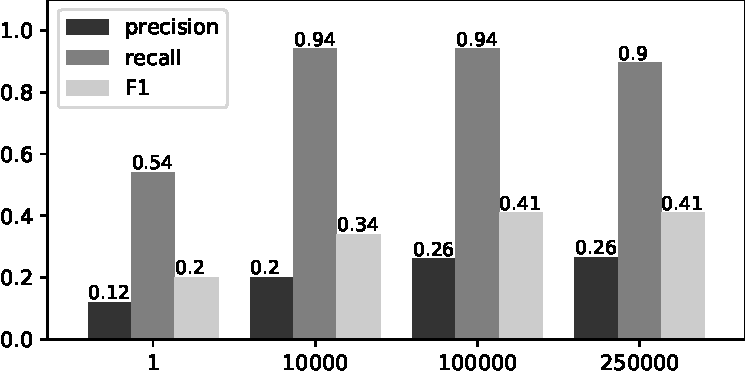
\includegraphics[width=\linewidth]{gfx/chap4/auxiliaryeffects.pdf}
\endminipage\hfill
\minipage{0.33\textwidth}
  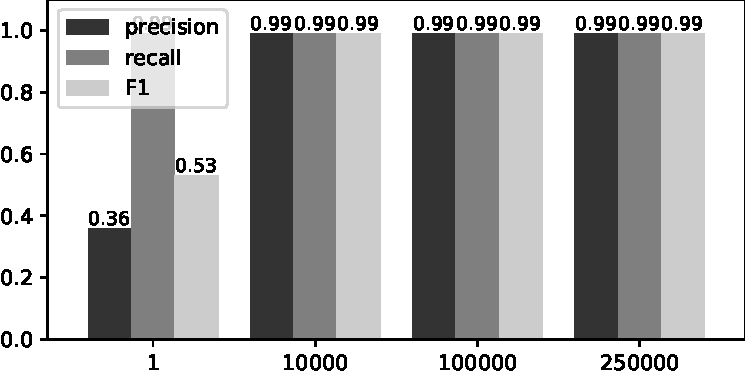
\includegraphics[width=\linewidth]{gfx/chap4/auxiliaryeffects_tbird.pdf}
\endminipage\hfill
\minipage{0.33\textwidth}
  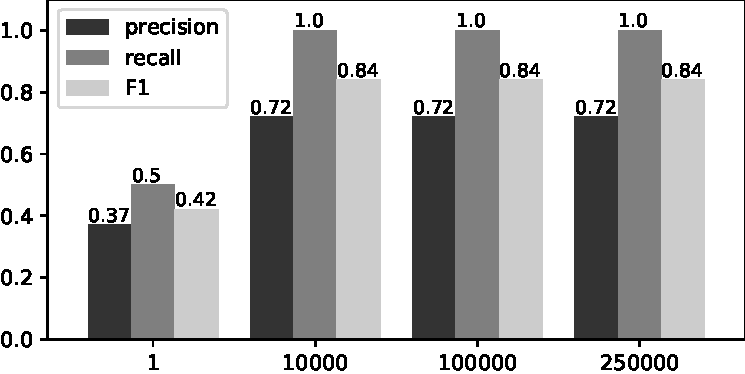
\includegraphics[width=\linewidth]{gfx/chap4/auxiliaryeffects_spirit.pdf}
\endminipage
\caption{Effect of the size of the auxiliary dataset. The target systems are Blue Gene/L, Thunderbird, and Spirit (left, middle, and right, respectively); 20\% train -- 80\% test split.}
\label{fig:auxiliary}
\end{figure*}

\subsubsection{Effect of the auxiliary data on the evaluation scores}
In this experiment, we perform an analysis of the Logsy performances with various sizes of the auxiliary data. We evaluate the same target vs. auxiliary data split for all datasets. We evaluate the approach on the 20\%--80\% train/test split. The results are shown in Figure~\ref{fig:auxiliary} for all datasets. The auxiliary data size increase from 1 to 250000 led to increases in all evaluation scores. With the increase in the size of the auxiliary data from 100000 to 250000, the scores do not change in both cases. This shows that the amounts of information present in the auxiliary data are similar and that all cases are already present in 100000 random samples. Notably, only one auxiliary sample, which may be even artificially generated, sufficiently acts as a regularizer to the hypersphere loss function. This prevents the model from learning trivial solutions. Increasing the variety of data (e.g., including more diverse log datasets) further improves the performance, owing to the increased number of samples representing abnormality.



% \begin{figure}[htbp]
%     \centering
%     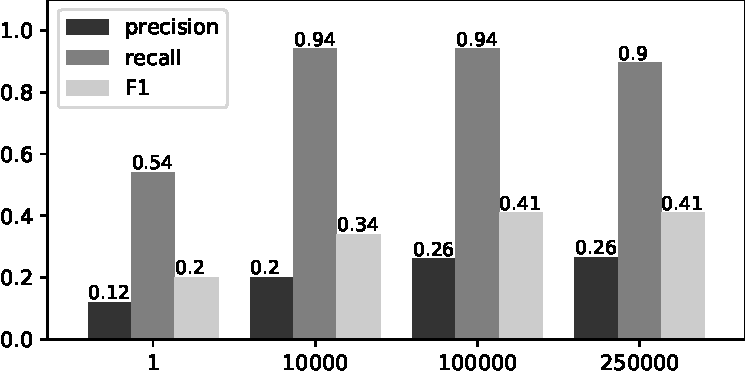
\includegraphics[width=0.99\columnwidth]{gfx/chap4/auxiliaryeffects.pdf}
%     \caption{Increasing the size auxiliary dataset, where the target system is the Blue Gene/L (20\% train - 80\% test)}
%     \label{fig:auxiliary_bgl}
% \end{figure}


% \begin{figure}[htbp]
%     \centering
%     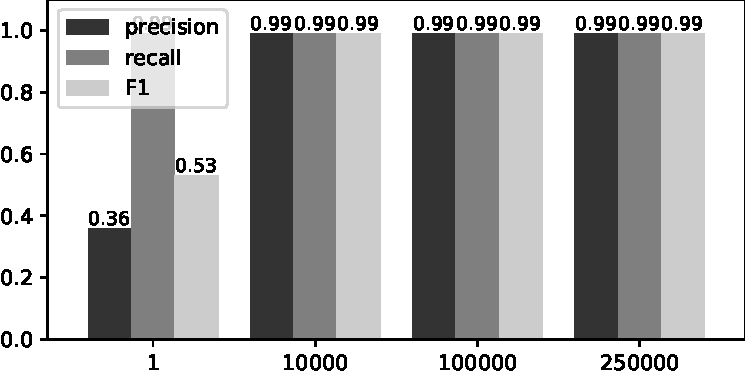
\includegraphics[width=0.99\columnwidth]{gfx/chap4/auxiliaryeffects_tbird.pdf}
%     \caption{Increasing the size auxiliary dataset, where the target system is the Thunderbird (20\% train - 80\% test)}
%     \label{fig:auxiliary_tbird}
% \end{figure}

% \begin{figure}[htbp]
%     \centering
%     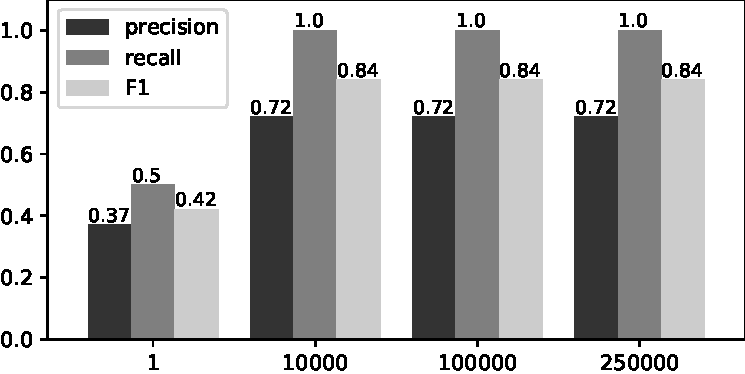
\includegraphics[width=0.99\columnwidth]{gfx/chap4/auxiliaryeffects_spirit.pdf}
%     \caption{Increasing the size auxiliary dataset, where the target system is the Spirit (20\% train - 80\% test)}
%     \label{fig:auxiliary_spirit}
% \end{figure}


\begin{figure}[!htbp]
\centering
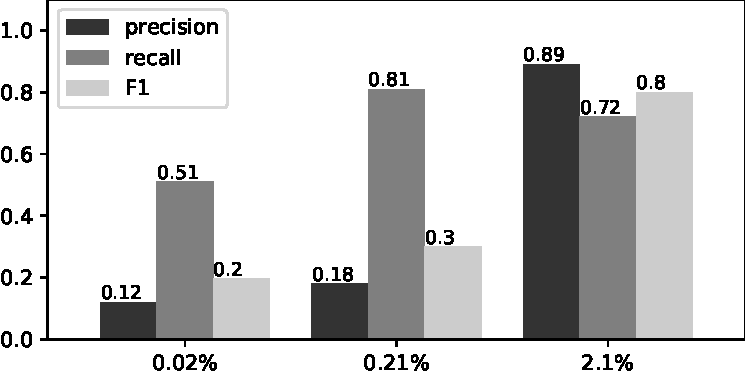
\includegraphics[scale=0.7]{gfx/chap4/semisupervised.pdf}
\caption{Effect of the increase in the size of the labeled anomaly data in the Blue Gene/L dataset (20\% train -- 80\% test).}
\label{fig:semisupervised}
\end{figure}


\subsubsection{Inclusion of expert labeling}
Often, systems are operated by humans, experts with system-specific knowledge. Sometimes, they could provide or manually label samples to improve the performance of the model. We experiment with the incremental inclusion of anomaly labels of the target dataset to test the model behaviour. We experiment on the 20\%--80\% split of the Blue Gene/L dataset. 
Figure~\ref{fig:semisupervised} shows the results. The increase in the number of labelled anomaly samples improves the performance. For as few as 2\% labelled data, we already obtain the best F1-score of 0.8. This shows that the addition of few percentages of anomalies as labelled samples to Logsy largely improves the performance. This only strengthens the hypothesis where the log anomaly detection must be addressed by understanding the reason responsible for the log message to be normal or anomalous. The labelled anomalies from the target system provide information utilized by Logsy to learn the differences between the normal and anomalous logs on the target dataset.


\begin{figure}[!b]
\centering
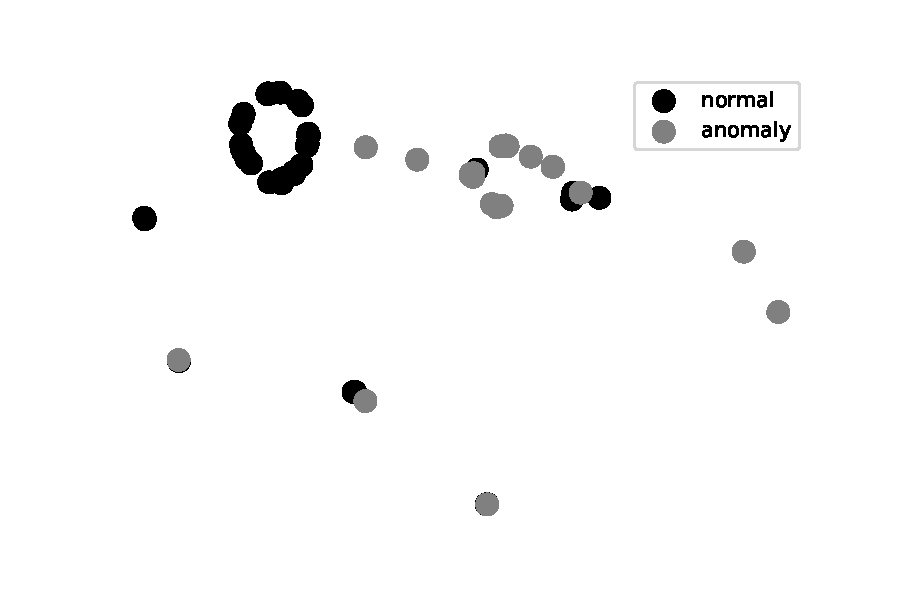
\includegraphics[scale=0.8]{gfx/chap4/tsne_BGL.pdf}
    \caption{Visualisations of the log vector representations of Blue Gene/L with T-SNE~\cite{maaten2008visualizing}.}
    \label{fig:tsne}
\end{figure}

\begin{figure}[!t]
\centering
   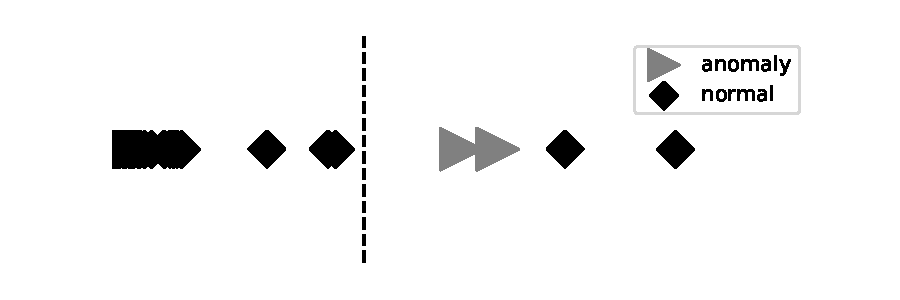
\includegraphics[scale=0.8]{gfx/chap4/thunderbird_distance.pdf}
    \caption{Distance of the log vector representations to the center of the hypersphere $\mathbf{c=0}$. The threshold is represented by the dashed line.}
    \label{fig:distance}
\end{figure}

\subsubsection{Utilization of the learned log embeddings in related approaches}
Representation learning is fundamental to obtain good performances of the machine learning methods~\cite{bengio2013representation}. In this experiment, we extract the learned log message vector representations from the already trained Logsy. To illustrate the vector representations of the logs, in Figure~\ref{fig:tsne}, we show their lower-dimensional representation of the test split through the T-SNE dimensionality reduction method~\cite{maaten2008visualizing} on the Blue Gene/L dataset. We show that the log vector representations are structured in a manner following the definition of our spherical loss function (see Section~\ref{vectorrepresentations}). The normal samples are concentrated around the centre of a hypersphere, which is a circle in two dimensions. Most of the anomalies are dispersed in the space outside the sphere. By assigning a threshold on the anomaly score $A(x_i)$, i.e., the distance from the centre of the sphere (circle), we can obtain a good performance. The same effect is observed on the Thunderbird dataset illustrated in Figure~\ref{fig:distance}, where we plot the distances of the test log vector representations to the centre of the sphere. The dashed line represents the optimal threshold for anomaly detection.  


\begin{figure}[!t]
    \centering
    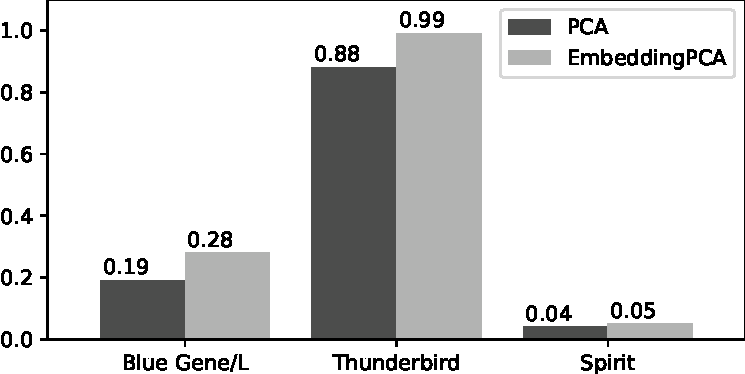
\includegraphics[scale=0.9]{gfx/chap4/pcaembeddings.pdf}
    \caption{F1 score comparison of the standard PCA~\cite{xu2009detecting} and PCA using the embeddings extracted from our method (80\%--20\% split).}
    \label{fig:pcaembeddings}
\end{figure}



To illustrate the importance of the log embeddings, we perform experiments where we replace the original TF-IDF log representations in PCA~\cite{xu2009detecting}, as the lowest-performance method, with the extracted embeddings from Logsy. We show the results in the bar plot in Figure~\ref{fig:pcaembeddings}. The replacement of the log representation improves the performance of the PCA. Improvements in F1 score of 0.09, 0.11, and 0.01 were obtained for Blue Gene/L, Thunderbird, and Spirit, respectively. This demonstrates that the log representation learning has an impact, not only in Logsy, but also in previous approaches that could be adapted to use the new log embeddings. The relative improvement in F1 score, on average, is 28.2\%.


\begin{figure*}[!htbp]
\minipage{0.5\textwidth}
  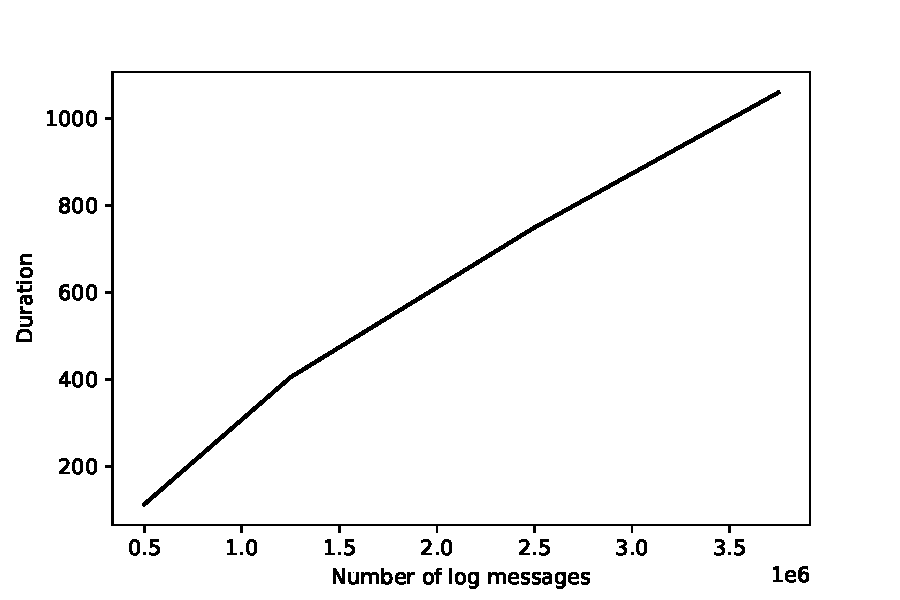
\includegraphics[width=1.0\textwidth]{gfx/chap5/logsyspeedgputrain.pdf}
\endminipage\hfill
\minipage{0.5\textwidth}
  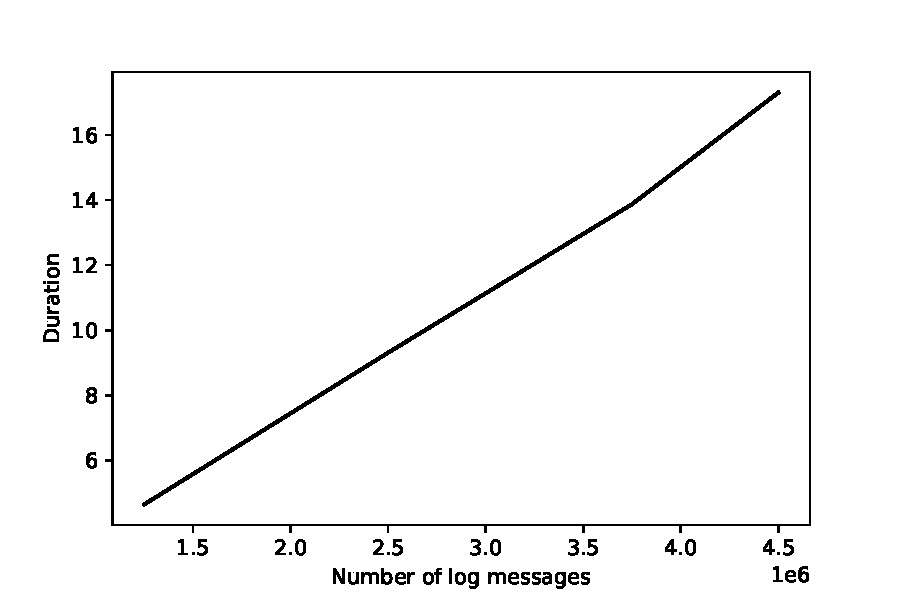
\includegraphics[width=1.0\textwidth]{gfx/chap5/logsyspeedgputest.pdf}
\endminipage
\caption{Speed performances of Logsy: training (left) and test (right) times.}
\label{fig:speedlogsy}
\end{figure*}


\subsubsection{Logsy: speed performance analysis}
To show that Logsy can be used in production in near-real-time settings, we evaluate its speed performance. The experiments were performed on a GPU NVIDIA 1660Ti (6GB) and CPU Intel(R) Core(TM) i7-9750H CPU at 2.60 GHz. Figure~\ref{fig:speedlogsy} shows the times needed for training and testing as functions of the data size. The figures show linear dependencies on the size of the log data. To analyze 3 million log lines, Logsy requires approximately 850 s for training and approximately 12 s for prediction. The prediction time is important in production settings, where less than $4 \mu s \mathrm{per log line}$ is required to predict each log line (obtained by dividing 12 s by 3 million log lines).


\section{Related work}
Extensive studies on the research and development of automated log analysis methods have been published in both industry and academia~\cite{zhu2019tools, he2016evaluation,shang2014log}. We provide an overview of the related studies on log parsing and log anomaly detection tasks.

\subsection{Log parsing}
Parsing techniques can be distinguished by various aspects, including technological, operation mode, and preprocessing. In Figure~\ref{fig:taxonomyparsing}, we present an overview of the existing methods.

\begin{figure}[htbp]
\centerline{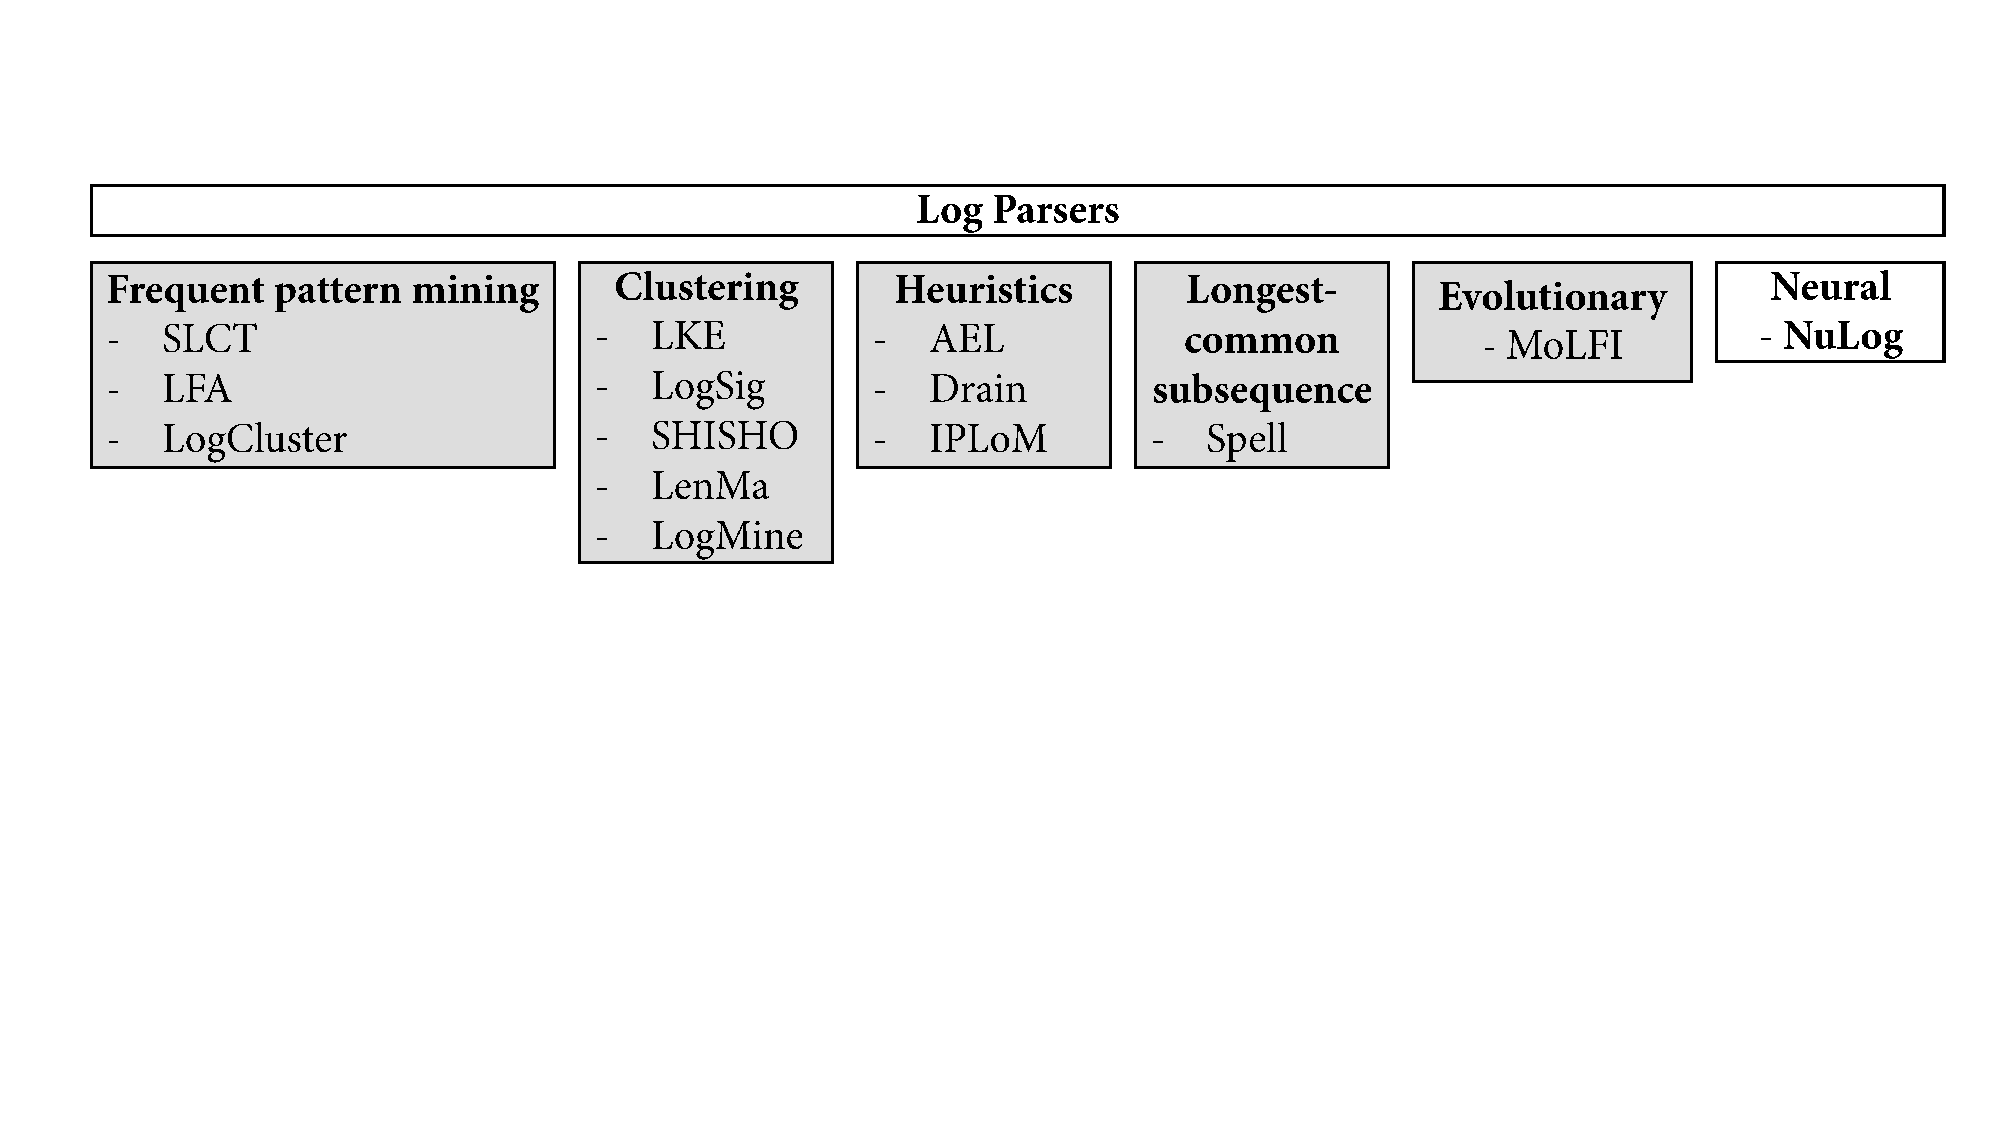
\includegraphics[width=1.0\textwidth]{gfx/chap4/figure_parser_taxonomy.pdf}}
\caption{Taxonomy of log parses according to the underlying technology.}
\label{fig:taxonomyparsing}
\end{figure}


\textbf{Clustering} The main assumption in these methods is that the message types coincide in similar groups. Various clustering methods with proper string matching distances have been used. Methods in this group include SHISO, LenMa, LogMine, LKE, LogSig~\cite{mizutani2013incremental, shima2016length,hamooni2016logmine, fu2009execution, tang2011logsig}. Other parsing methods such as POD-Discovery~\cite{imweber2015}, are found in process mining, which utilize regular expressions and leverages the Levenshtein distance to separate variable and constant parts of the logs.

\textbf{Frequent pattern mining} assumes that a message type is a frequent set of tokens that appear throughout the logs. The procedures involve creating frequent sets, grouping the log messages, and extraction of message types. Representative parsers for this group are SLCT, LFA, and LogCluster~\cite{xu2009detecting, nagappan2010abstracting, nandi2016anomaly}.


\textbf{Evolutionary}. Its member MoLFI~\cite{messaoudi2018search} uses an evolutionary approach to find the Pareto optimal set of message templates.

\textbf{Log-structure heuristic methods} produce the best results among the different used techniques~\cite{zhu2019tools,he2016evaluation}. They usually utilize different properties that emerge from the structure of the log. The state-of-the-art algorithm Drain~\cite{he2017drain} assumes that, at the beginning of the logs, the words do not largely vary. It uses this assumption to create a tree with a fixed depth, which can be easily modified for new groups. In this group there are as well other related parsers such as IPLoM, and AEL~\cite{xu2009detecting, jiang2008automated}.

\textbf{Longest common subsequence} uses the longest common subsequence algorithm to dynamically extract log patterns from incoming logs. The most representative parser is Spell~\cite{du2016spell}.

The proposed method NuLog belongs to a new category referred to as \textbf{Neural} in the taxonomy of log parsing methods. Different from the current state-of-the-art heuristic-based methods, our method does not require any domain knowledge. Through empirical results, we show that the model is robust and applicable to various log types in different systems.

\subsection{Log anomaly detection}

Similarly to the log parsing, extensive studies have been published on the research and development of methods for log anomaly detection in both industry and academia~\cite{bodik2010fingerprinting, jakublogs,chen2004failure,farshchi2015experience,fu2009execution, hamooni2016logmine, liang2007failure, du2017deeplog, xu2009detecting,  zhang2019robust, meng2019loganomaly, nedelkoski2020selfsupervised,xu2014weber}. Out of those, the older methods utilize traditional statistical and machine learning models, and human intervention in the model creation, while the current studies focus on utilizing the large amounts of log data and mostly apply deep learning models.

Numerous supervised methods have been applied to address the log anomaly detection problem. For example, Liang et al.~\cite{liang2007failure} applied a support vector machine (SVM) classifier to detect failures, where both normal and anomalous samples are assumed to be available. Similarly, Chen et al.~\cite{chen2004failure} utilized the decision tree to model the logs from the targeted application. 
Brier et al.~\cite{breier2015anomaly} provided an overview of these supervised and more traditional approaches to log anomaly detection. Recently, LogRobust~\cite{zhang2019robust} and HitAnomaly~\cite{huang2020hitanomaly} provided supervised methods on sequences of log data and state-of-the-art results. However, as explained above, obtaining system-specific labeled samples is costly and often practically infeasible. Therefore, we discuss unsupervised methods below.

Several unsupervised learning methods have been proposed. Xu et al.~\cite{xu2009detecting} proposed using the PCA method, where they assumed different sessions in a log file that can be easily identified by a session-id attached to each log entry. It groups log keys by session, and then counts the appearances of each log key value inside each session. A session vector has a size of $n$, representing the number of appearances for each log key in $K$ in that session. A matrix is formed where each column is a log key, while each row is one session vector. PCA detects an abnormal vector (a session) by measuring the projection length on the residual subspace of a transformed coordinate system. The publicly available implementation enables a TF-IDF representation of the log messages, which is utilized in our experiments as a baseline. Lou et al.~\cite{lou2010mining} proposed invariant mining (IM) to mine the linear relationships among log events from log event count vectors. 

Log anomaly detection methods based on one-class classification~\cite{Zhang2016AutomatedIS,Vinayakumar2017LongSM} learn a model that describes the normal system behavior, usually assuming that most of the unlabeled training data are not anomalous and that anomalies are samples outside the learned decision boundary. The massive log data volumes in large systems have renewed the interest in the development of one-class deep learning methods to extract general patterns from nonanomalous samples. We classify these methods into the traditional group of methods, which leverage log parsing~\cite{nedelkoski2020selfsupervised, he2017drain} and follow the traditional log anomaly detection pipeline described in Figure~\ref{fig:parsingreferenceanomaly}. The formulated task is to predict the next index of the log template in the sequence $x_{h+1}$ by utilizing the history of template vectors (count, one-hot encoding) $H=x_0,\dots,x_h$, as for DeepLog~\cite{du2017deeplog}.

Some studies have leveraged NLP techniques to analyze log data based on the fact that log is a natural language sequence. Zhang et al.~\cite{Zhang2016AutomatedIS} proposed to use the LSTM model and TF-IDF weight to predict the anomalous log messages. Bertero et al.~\cite{bertero2017experience} used word2vec and traditional classifiers, such as SVM and Random Forest, to evaluate whether a log event is an anomaly. Similarly, LogAnomaly~\cite{meng2019loganomaly} incorporates pretrained word vectors for learning of a sequence of logs; they trained an attention-based Bi-LSTM model.

Furthermore, in the process-based modelling literature there are number of methods that also consider anomaly detection from log data as sequential problem. Xu et al.~\cite{xu2014weber} use log data to extract operational activities such as upgrade, redeployment, and on-demand scaling and perform anomaly detection to increase the system dependability. The authors proposed Process Oriented Dependability (POD)-Diagnosis, an approach that explicitly models these
sporadic operations as processes. These models allow to determine orderly execution of the process, use the process context to filter logs, trigger assertion evaluations, visit
fault trees, and perform on-demand assertion evaluation for online anomaly detection. In the same direction, several other studies from process-based anomaly detection~\cite{nolle2020process,PECCHIA2020105054,nolle2016unsupervised,nolle2018analyzing,nolle2019binet,imweber2015,xu2014weber,rehse2020} make use of sequential log events to mine processes and detect anomalies. In these studies, log data is often associated with having trace ID, where log events are related, and activities are extracted to bridge the gap from raw log events to the process mining methods. On the other hand, we view the log events as independent samples, and analyze them from the point of natural language processing, and text anomaly detection. We draw more concrete comparison to these methods in the trace analysis chapter.

The learning of the sequence of template indices and enhanced log message embedding approaches still have large limitations in terms of generalization for previously unseen log messages. They tend to produce false predictions owing to the imperfect log vector representations. For example, learning sequence of logs represented by indices cannot correctly classify newly appearing log messages, as the new log will be an out-of-boundary index. The domain where the word vectors are pretrained (e.g., Wikipedia) has essential differences from the language used in computer system development. To partly mitigate some of these limitations in unsupervised approaches, one approach is to incorporate labeled data from operators and perform life-long learning~\cite{du2019lifelong}. However, it still requires frequent periodical retraining, updates, and costly expert knowledge to label the data, without addressing the problem of generalization on unseen log messages that appear between retraining epochs. 

Different from the above methods, we used the interpretation of the anomaly detection as binary classification between normal and anomalous points. We utilized the concept reported by Steinwart et al.~\cite{steinwart2005classification} that the bias on the anomalous distribution is crucial for an improved detection. We provided such bias by employing easily accessible log datasets as an auxiliary data source. 

\section{Chapter summary} \label{conclusion}
Logs are an important data source for anomaly detection in computer systems~\cite{zhu2019tools, du2017deeplog, zhang2019robust}. In this chapter, we described the traditional pipeline for log anomaly detection. Most methods utilize log parsing as the first step toward anomaly detection. We identified limitations in existing parsing methods, including the use of regular expressions, heuristics (e.g., the variable parts of the log message appear near the end of the log message~\cite{he2017drain}), and multiple hyperparameters for tuning~\cite{zhu2019tools,du2016spell,hamooni2016logmine}. As the anomaly detection depends on the parsing, the accuracy of the log parsing directly affects the effectiveness of the log anomaly detection. Therefore, we presented a method, NuLog, to mitigate these limitations and improve the overall effectiveness of the methods. NuLog addressed the log parsing problem by deep language modelling. Words appearing at a constant position of a log record implies that their correct prediction can be directly used to produce a log message type. An incorrect prediction indicates that a token is a parameter. 
We carried out experiments on 10 real-world log datasets and evaluated the method against 12 log parsers from a public benchmark. The experimental results showed that NuLog outperforms the existing log parsers in terms of accuracy, edit distance, and robustness. In addition to the parsed templates, NuLog produces log vectors. We analyzed the effectiveness of using the log vectors directly for anomaly detection. In the analysis, we compared the NuLog log vectors with the state-of-the-art log anomaly detection method and anomaly detector trained in a supervised manner. The NuLog's log vectors improve the anomaly detection. However, we identified a large gap between the efficiency scores, favoring the supervised learning. The unsupervised approaches still led to large numbers of FPs. 

To bridge the gap between supervised and unsupervised anomaly detection methods, we identified the log vectors as a main issue in previous methods~\cite{he2017drain,du2016spell,meng2019loganomaly,zhang2019robust,du2017deeplog}. The main drawback is the prediction of unseen log messages owing to the evolution of logging statements, system updates, and processing noise. 

To overcome this problem, we presented a new anomaly detection approach, Logsy. Logsy shifts from the traditional log anomaly detection pipeline and does not utilize an external log vector computation. In contrast, it learns end-to-end log vectors and predicts anomaly scores. It is based on a self-attention encoder network with a new hyperspherical classification objective. We formulated the log anomaly detection problem in a manner to discriminate between normal training data from the system of interest and samples from auxiliary easy-access log datasets from other systems, which represent an abnormality.

We presented an experimental evidence that our classification-based method Logsy exhibits a high performance for deep anomaly detection. Logsy outperformed the baselines by an F1 score margin of 0.25. Logsy can efficiently include available expert labels. Furthermore, the log vector representations from Logsy are meaningful and generally can be utilized in other methods. Using PCA to utilize the log vectors from Logsy, we obtained an improvement in the F1 score of 0.07 (28.2\%). 

The preference for unsupervised learning in previous log anomaly detection studies is reasonable for the traditional settings, which often lack access to out-of-distribution samples that are representative examples of anomalous data. Owing to the large amount of easily obtainable log data, it is reasonable to assume that access to anomaly data informative for detection is available. We hypothesize that future research on deep log anomaly detection should focus on classification with anomalous auxiliary data and development of approaches to incorporate domain bias for the diversity of normal and anomaly data. 

